\RequirePackage{ifpdf}
\documentclass[letterpaper,landscape]{slides}
%\documentclass[letterpaper,portrait]{slides}
\usepackage{boxedminipage}
\usepackage{amsmath}
\usepackage{amssymb}
\usepackage{bm}

%\input /u/rhl/TeX/pdf.tex
\input pdf.tex

\newif\ifTalk\Talktrue		% We generating a talk, not printing
%\Talkfalse			% no; we're really printing

%\pagestyle{empty}
\setlength{\topmargin}{-1in}
\setlength{\textheight}{7.5in}
\setlength{\textwidth}{9in}
\setlength{\oddsidemargin}{0pt}
\setlength{\oddsidemargin}{0pt}

%\onlyslides{1-3,4,10-9999}
%\onlyslides{26-9999}

\begin{document}

\newcommand{\XXX}[1]{\textbf{XXX} #1}
\newcommand{\colour}[1]{\color{#1}}

\def\eq#1{\begin{equation} \color{blue} #1 \end{equation}}
\def\vx{{\bf x}}
\def\vv{{\bf v}}
\def\p{\partial}
\def\b#1{{\bf  #1}}
\def\p{\partial}
\def\th{^{th}}
\def\msun{{\rm\,M_\odot}}
\def\bnabla{{\bf\nabla}}
\def\dint{\int\!\!\!\int}
\def\d{{\rm d}}
\def\i{{\rm i}}
\def\ddt#1{{\rm{d} #1\over {\rm dt}}}
\def\ddtS#1{{\rm{d^2} #1\over {\rm dt^2}}}
%\lta and \gta produce > and < signs with twiddle underneath
\def\spose#1{\hbox to 0pt{#1\hss}}
\def\lta{\mathrel{\spose{\lower 3pt\hbox{$\mathchar"218$}}
     \raise 2.0pt\hbox{$\mathchar"13C$}}}
\def\gta{\mathrel{\spose{\lower 3pt\hbox{$\mathchar"218$}}
     \raise 2.0pt\hbox{$\mathchar"13E$}}}
\def\mspace{\hbox{\quad}}
\def\deffn#1{{\bf#1}}\def\eqs#1{equations \rf#1}






\newcount\itemCnt\itemCnt=0
\newcommand{\nitem}{%
  \global\advance\itemCnt by 1
  ~\vskip0cm\the\itemCnt.\qquad}

\definecolor{orange}{rgb}{1.0, 0.5, 0.0}
\definecolor{purple}{cmyk}{0.4, 0.8, 0.3, 0.0}


%%%%%%%%%%%%%%%%%%%%%%%%%%%%%%%%%%%
\newcommand{\onepic}[6]{%
\begin{slide}
     \begin{center}
        \begin{minipage}{#1in}
            {\large \color{blue} #6}
            \phantom{x} \vskip #2in
            \phantom{x} \hskip #3in
            {\scalebox{#4}{\includegraphics{#5}}}   
        \end{minipage}
     \end{center}
    \vfill
\end{slide}
}


%%%%%%%%%%%%%%%%%%%%%%%%%%%%%%%%%%%
\newcommand{\picslide}[7]{%
  \begin{slide}
     \begin{center}
        \begin{minipage}{#5in}
            \hskip #6in
            \hskip -1in
            {\scalebox{#4}{\includegraphics{#1.#2}}}
            \vskip #7in~
            {\large \color{blue} #3}
        \end{minipage}
     \end{center}
     \vfill
  \end{slide}
}
%%%%%%%%%%%%%%%%%%%%%%%%%%%%%%%%%%%
 

%%%%%%%%%%%%%%%%%%%%%%%%%%%%%%%%%%%
\newcommand{\Spicslide}[7]{%
  \begin{slide}
     \begin{center}
        \begin{minipage}{#5in}
            \vskip #6in
            \hskip #7in
            {\scalebox{#4}{\includegraphics{#1.#2}}}
        \end{minipage}
     \end{center}
     \vfill
  \end{slide}
}
%%%%%%%%%%%%%%%%%%%%%%%%%%%%%%%%%%%
 



%------------------------------------------------------------------------------

\begin{slide}

\phantom{x}
\vskip -2in
\begin{center}
\bfseries
{\large {\color{blue} Astr 511: Galaxies as galaxies}}
\end{center}

{\centerline {{\color{blue} 
Winter Quarter 2017, University of Washington}}}
{\centerline {{\color{blue} 
Mario Juri\'{c} \& \v{Z}eljko Ivezi\'{c} }}}

\vskip 1.6in

{\centerline {\huge {\color{red}      Lecture 9:             }}}
\vskip 0.2in 
{\centerline {\Large {\color{blue} Dynamics IV: Dynamics of Disks, }}}
\vskip 0.1in
{\centerline {\Large {\color{blue} Spiral Structure, and Bars }}}

\vfill
\end{slide}
%------------------------------------------------------------------------------


%------------------------------------------------------------------------------
\begin{slide}
\vskip 4.5in
\begin{center}
{\large \color{red} 
                  Disk Dynamics and Spiral Structure   }
\end{center}

So far, we've studied the dynamics that helps explain morphology and
kinematics of early type galaxies.  In these explorations, we've modeled
galaxies as spheroids or somewhat flattened axisymmetric, collisionless,
systems.  This has worked wonderfully in explaining the phenomenology
of ETGs and providing some insight of the physics that underpins them.

However, we know that not all galaxies can be modeled as spheroids. A
significant fraction (including the Milky Way) are characterized by 
(thin) disks and asymmetric features such as {\bf spirals} and {\bf bars}.

In this lecture, we'll examine the phenomoenology of these, mostly late
type, galaxies and introduce the dynamical framework that allows us to
understand them.

\vskip 0in

\begin{flushright}
{ \tiny - Binney \& Tremaine, \S6. } \\
\end{flushright}

\end{slide}

%------------------------------------------------------------------------------
\begin{slide}
\begin{center}
\vskip 3in
{\large \color{red} Phenomenology of Spiral Structure  }
\end{center}

\end{slide}


%------------------------------------------------------------------------------
\begin{slide}
\begin{center}
{\large \color{red} 
                  Messier 100 (Sbc)  }
\end{center}

\begin{center}
\vskip -0.0in
\scalebox{0.50}{\hskip 0.0in 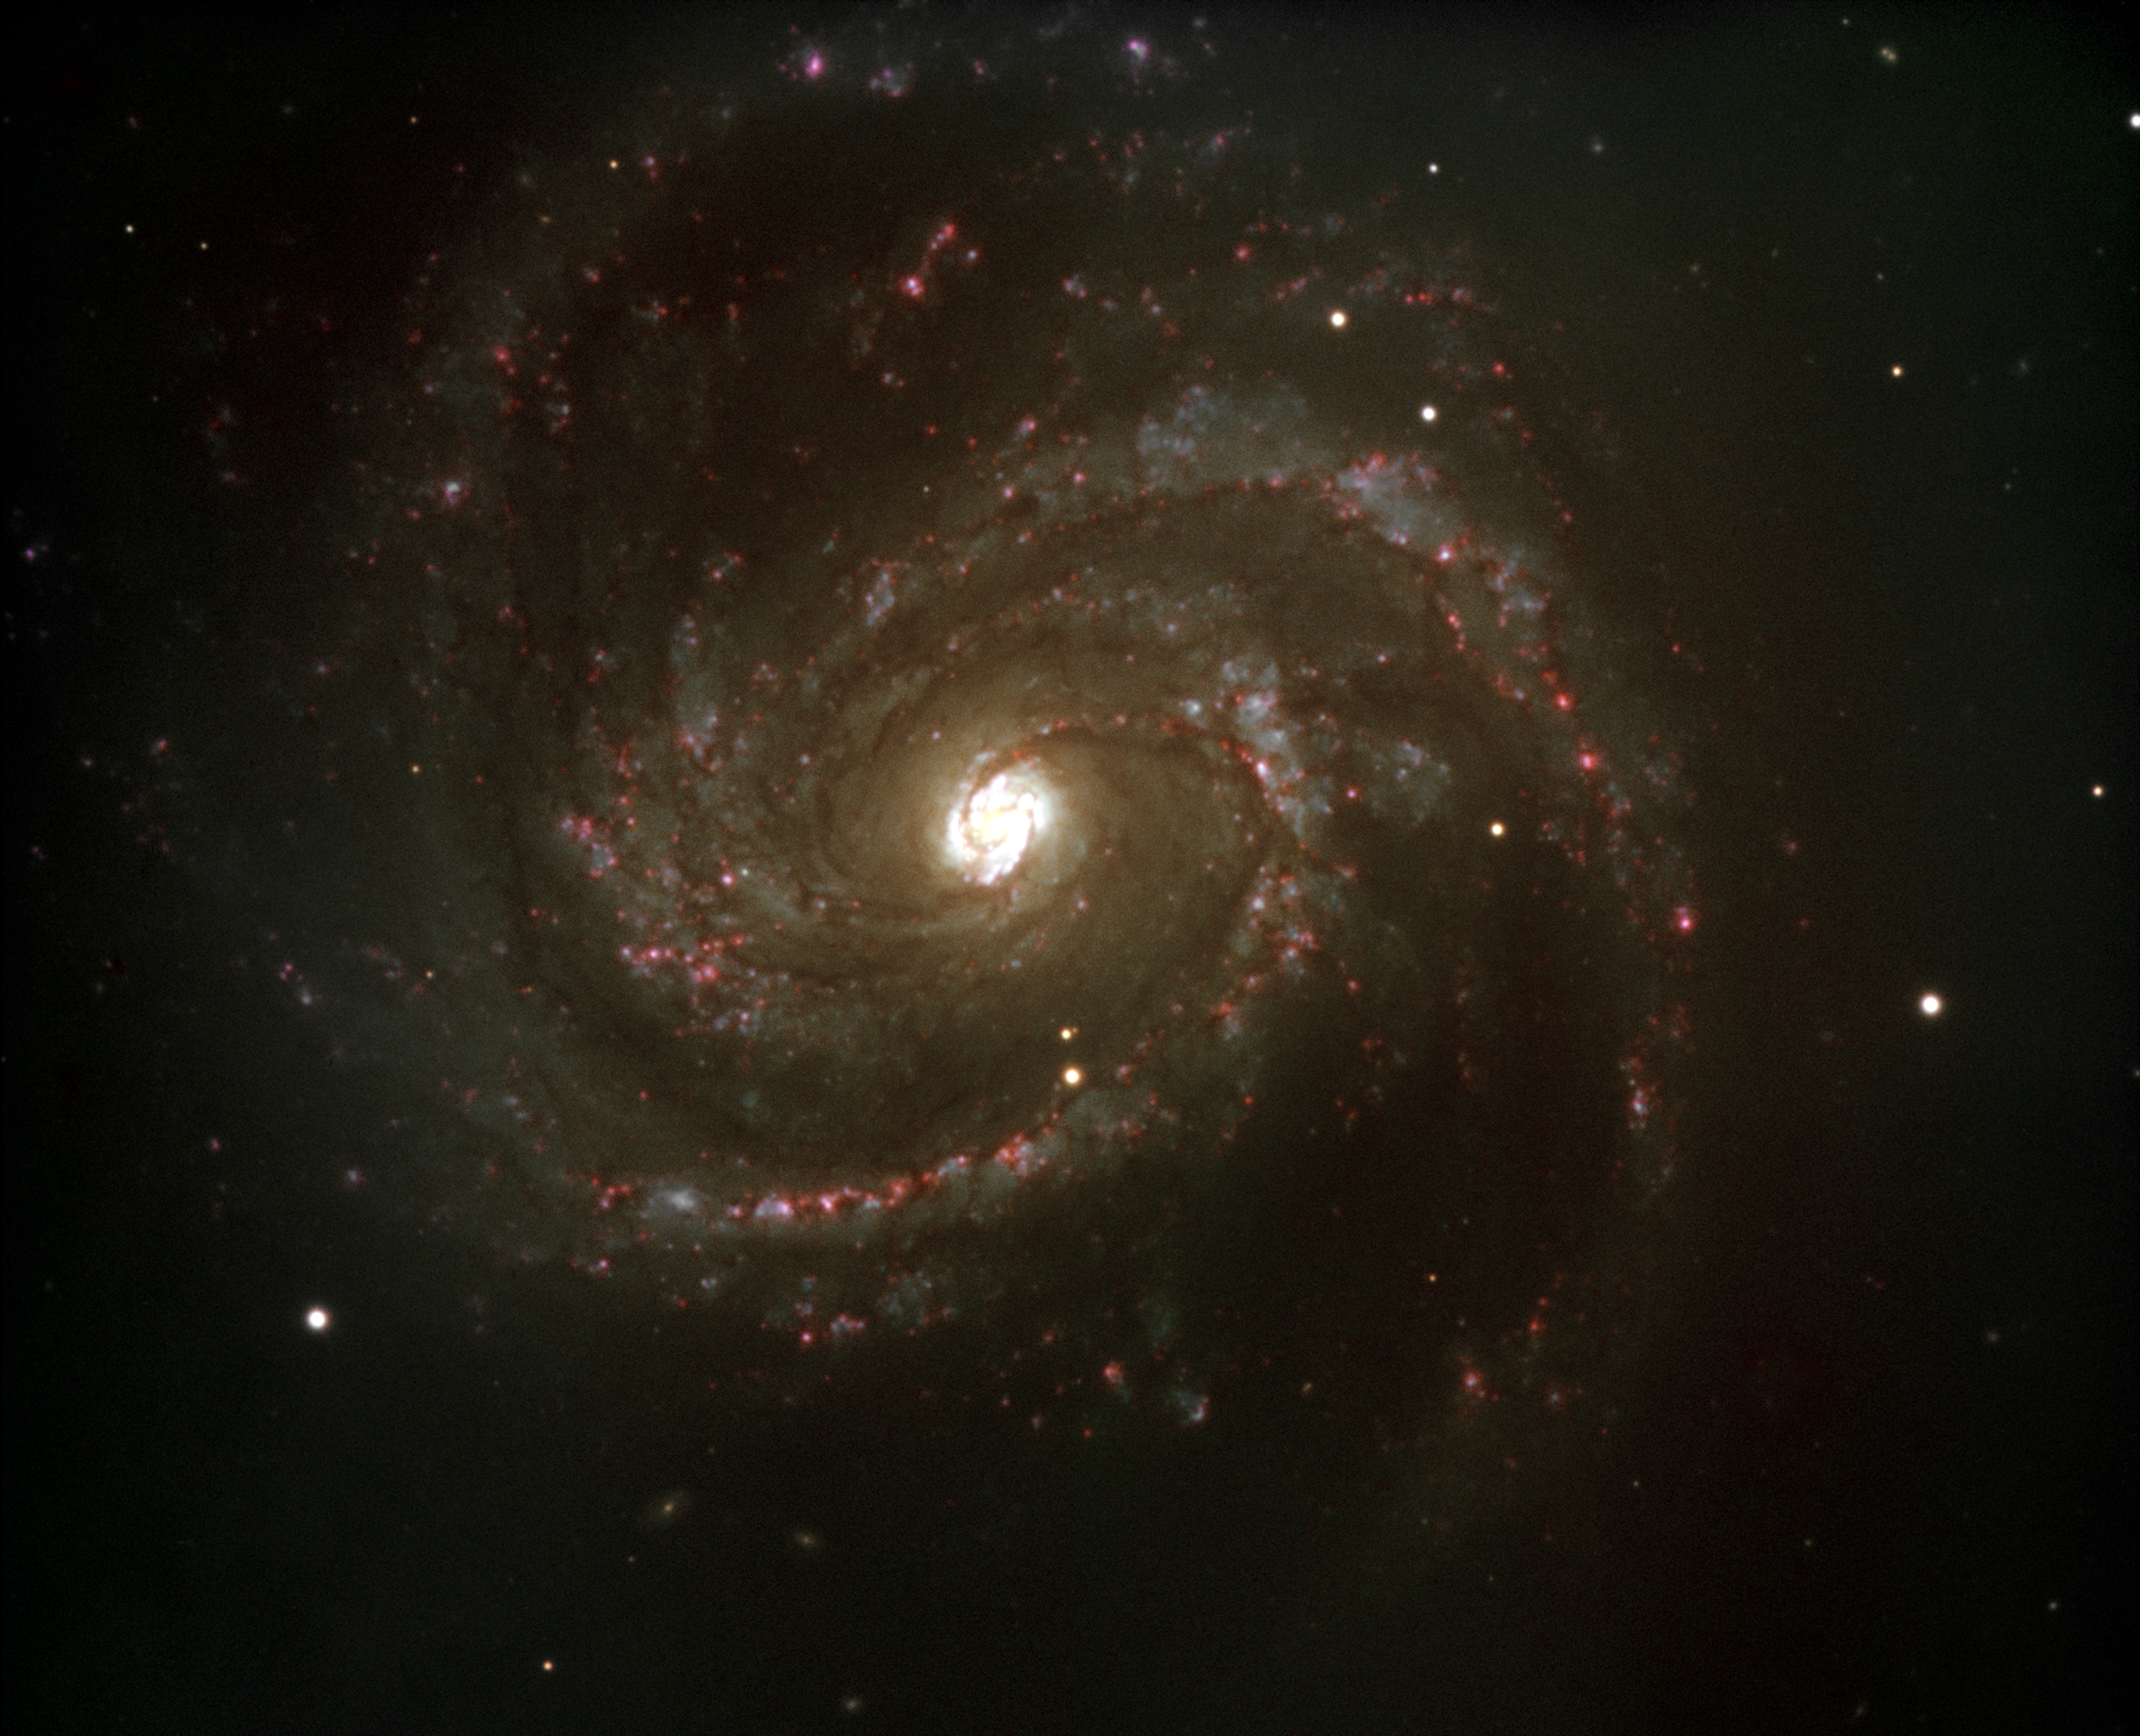
\includegraphics{figures/M100}}
\end{center}

\begin{flushright}
{ \tiny \em -- European Southern Observatory }
\end{flushright}

\vfill
\end{slide}


%------------------------------------------------------------------------------
\begin{slide}
\begin{center}
{\large \color{red} 
                  Messier 101 (Sc)  }
\end{center}

\begin{center}
\vskip -0.0in
\scalebox{0.27}{\hskip 0.0in 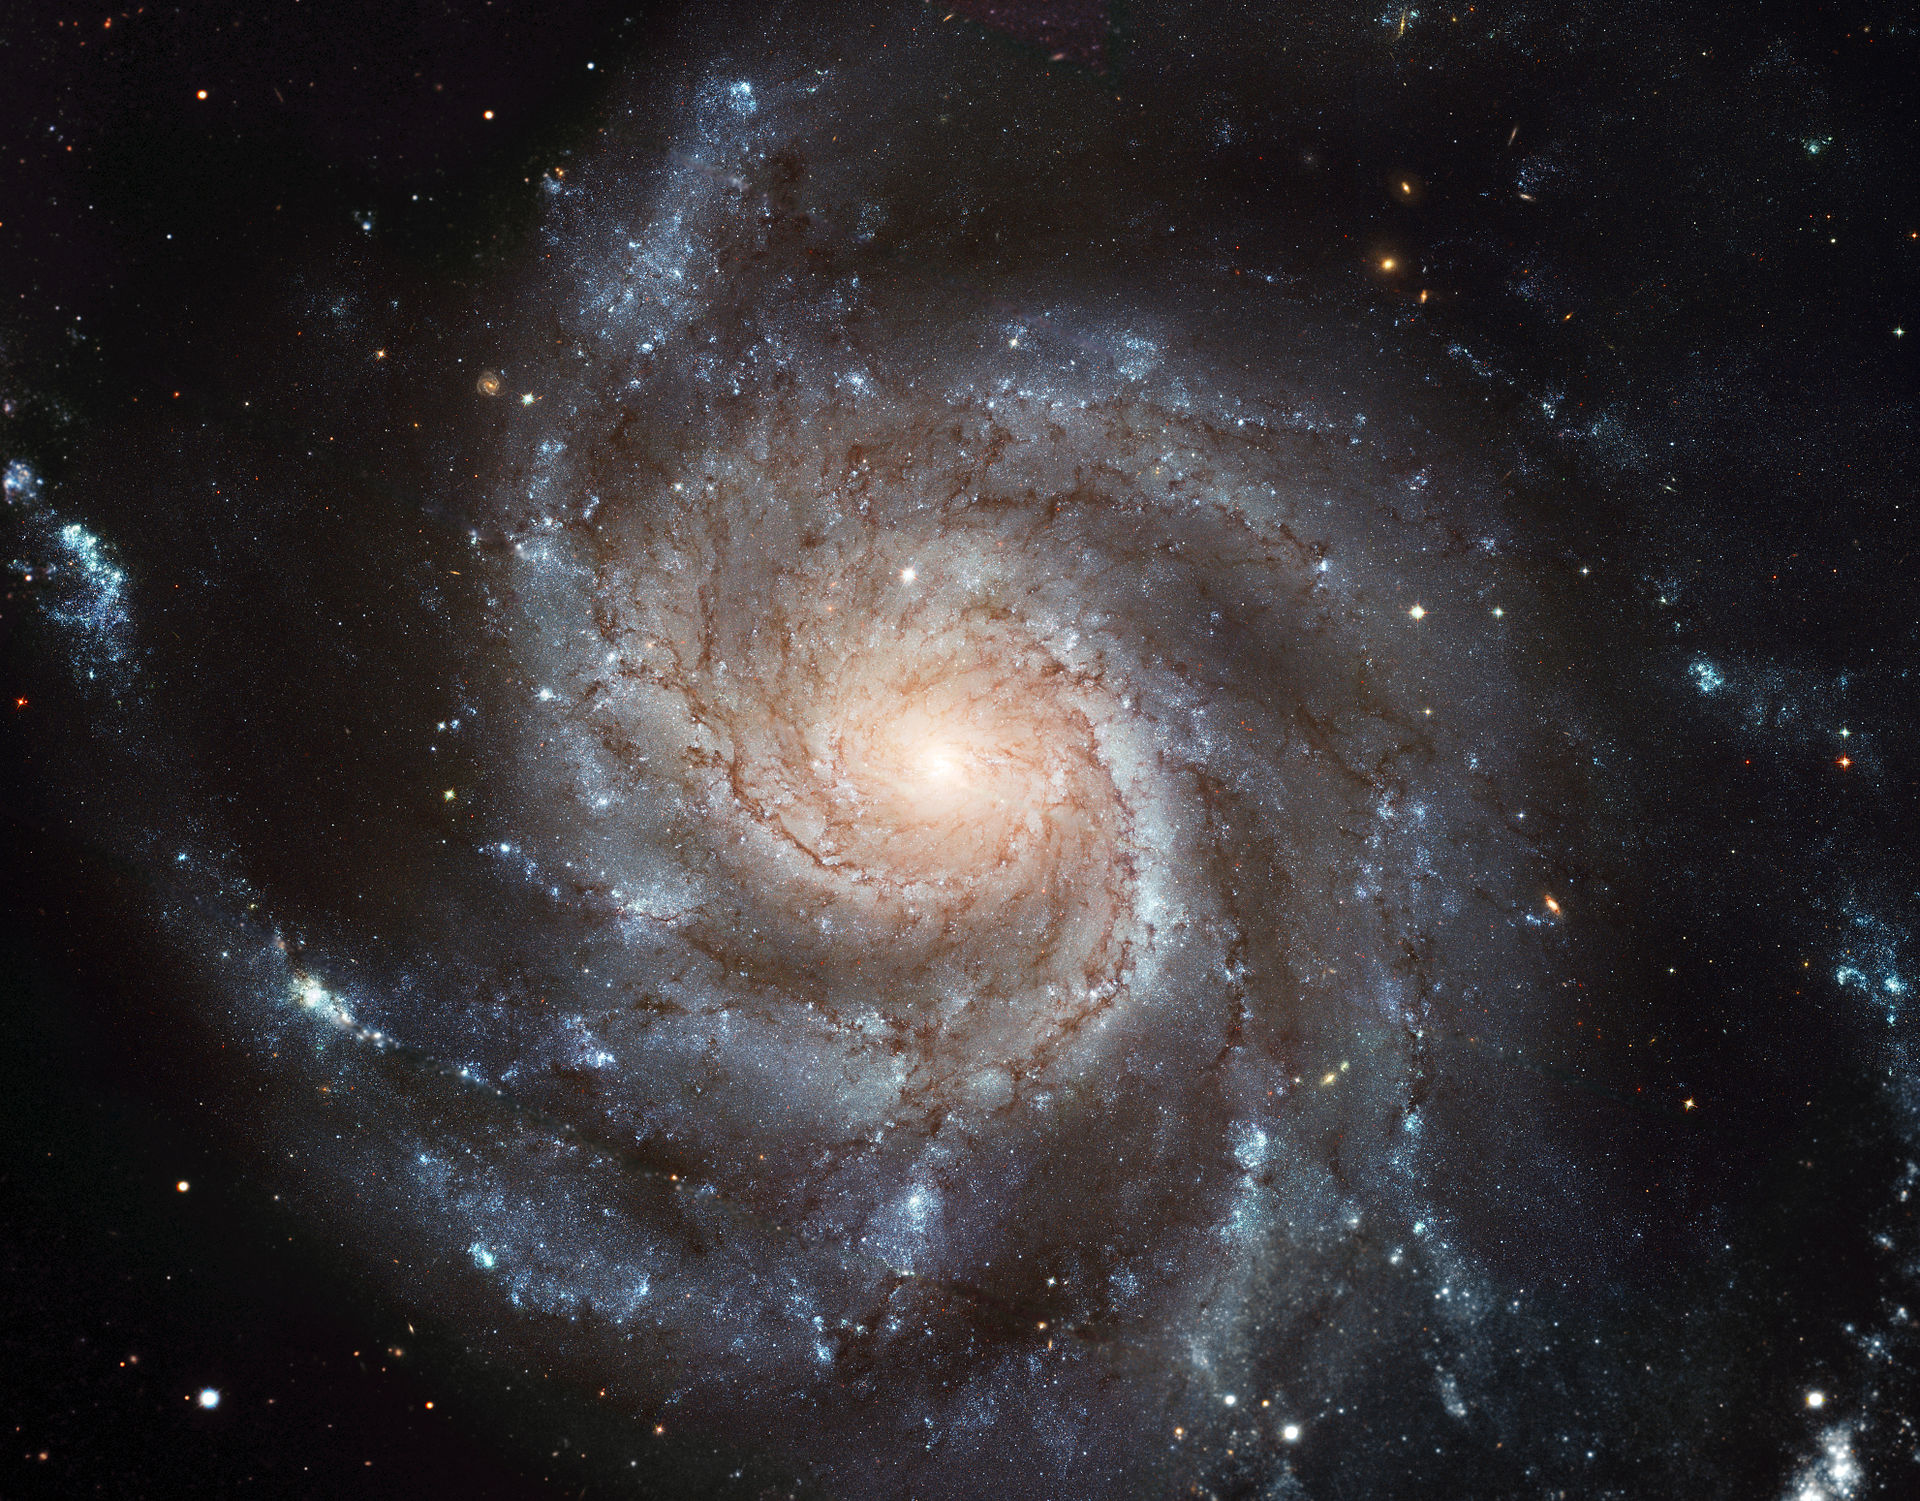
\includegraphics{figures/M101_hires_STScI-PRC2006-10a-small.jpg}}
\end{center}

\begin{flushright}
{ \tiny \em -- HST/STScI/NASA }
\end{flushright}

\vfill
\end{slide}


%------------------------------------------------------------------------------
\begin{slide}
\begin{center}
{\large \color{red} 
                  Messier 33 (Scd)  }
\end{center}

\begin{center}
\vskip -0.0in
\scalebox{0.25}{\hskip 0.0in 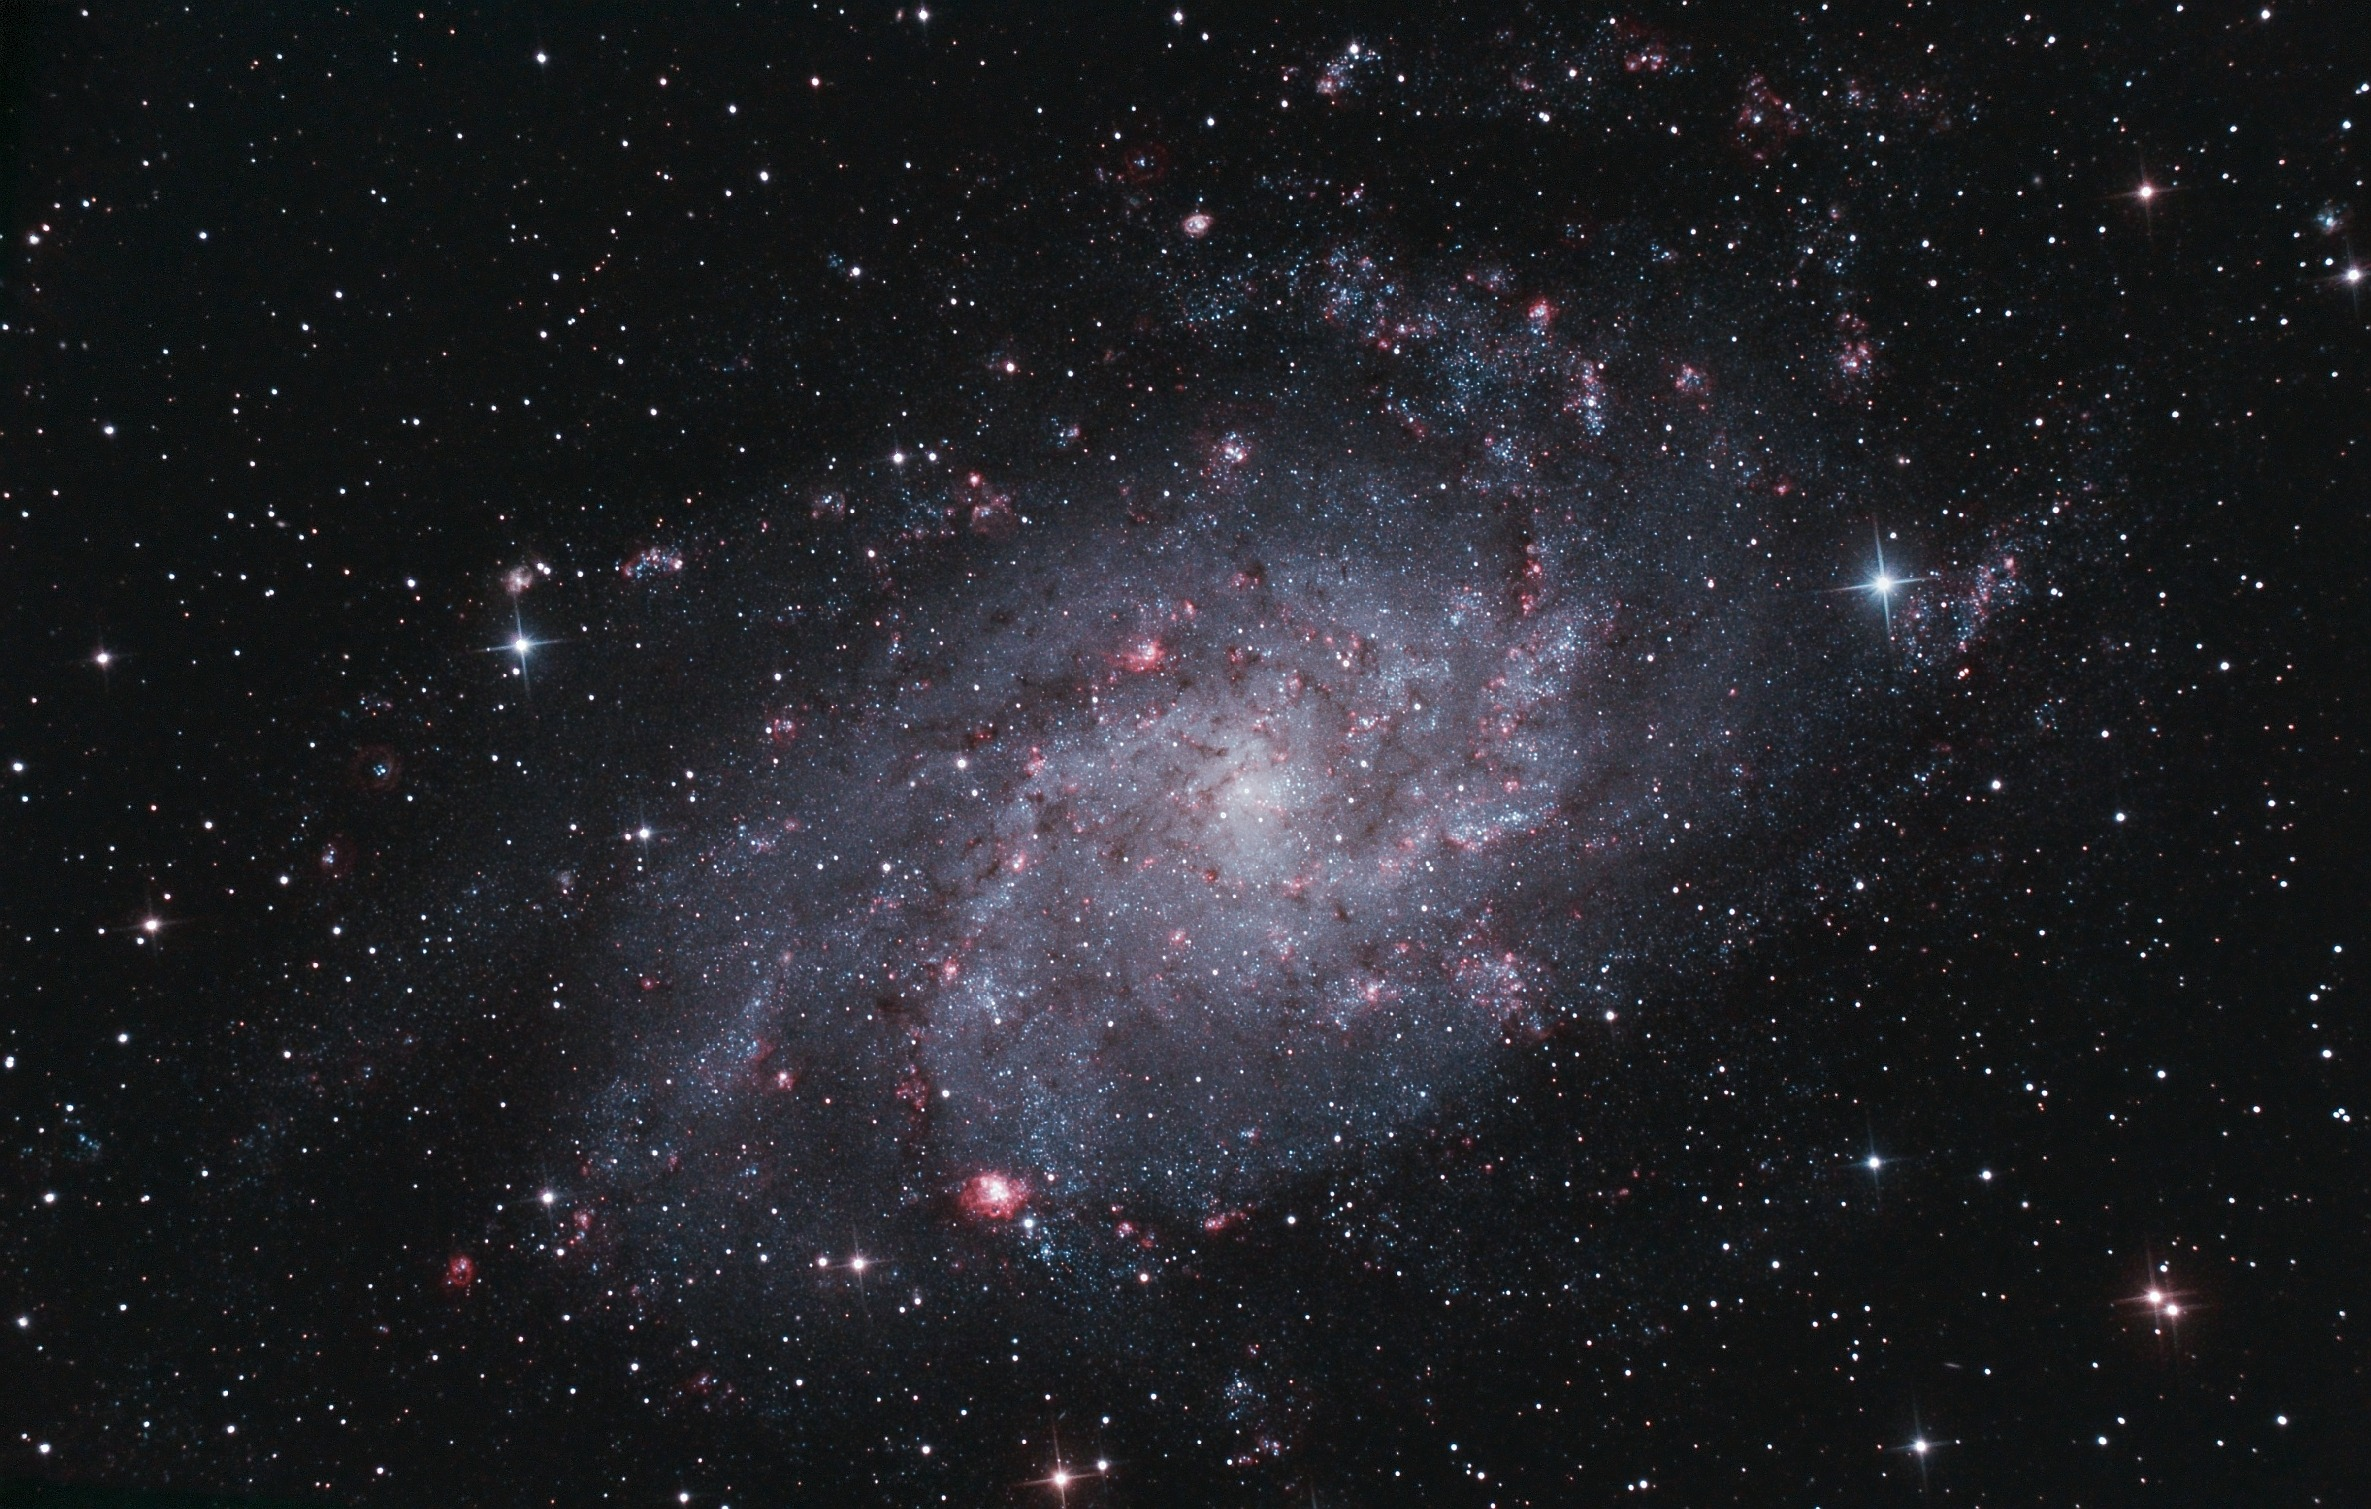
\includegraphics{figures/M33_-_Triangulum_Galaxy}}
\end{center}

\begin{flushright}
{ \tiny \em -- (c) Alexander Meleg }
\end{flushright}

\vfill
\end{slide}


%------------------------------------------------------------------------------
\begin{slide}
\begin{center}
{\large \color{red} 
                  Messier 63 (Scb)  }
\end{center}

\begin{center}
\vskip -0.0in
\scalebox{1.0}{\hskip 0.0in 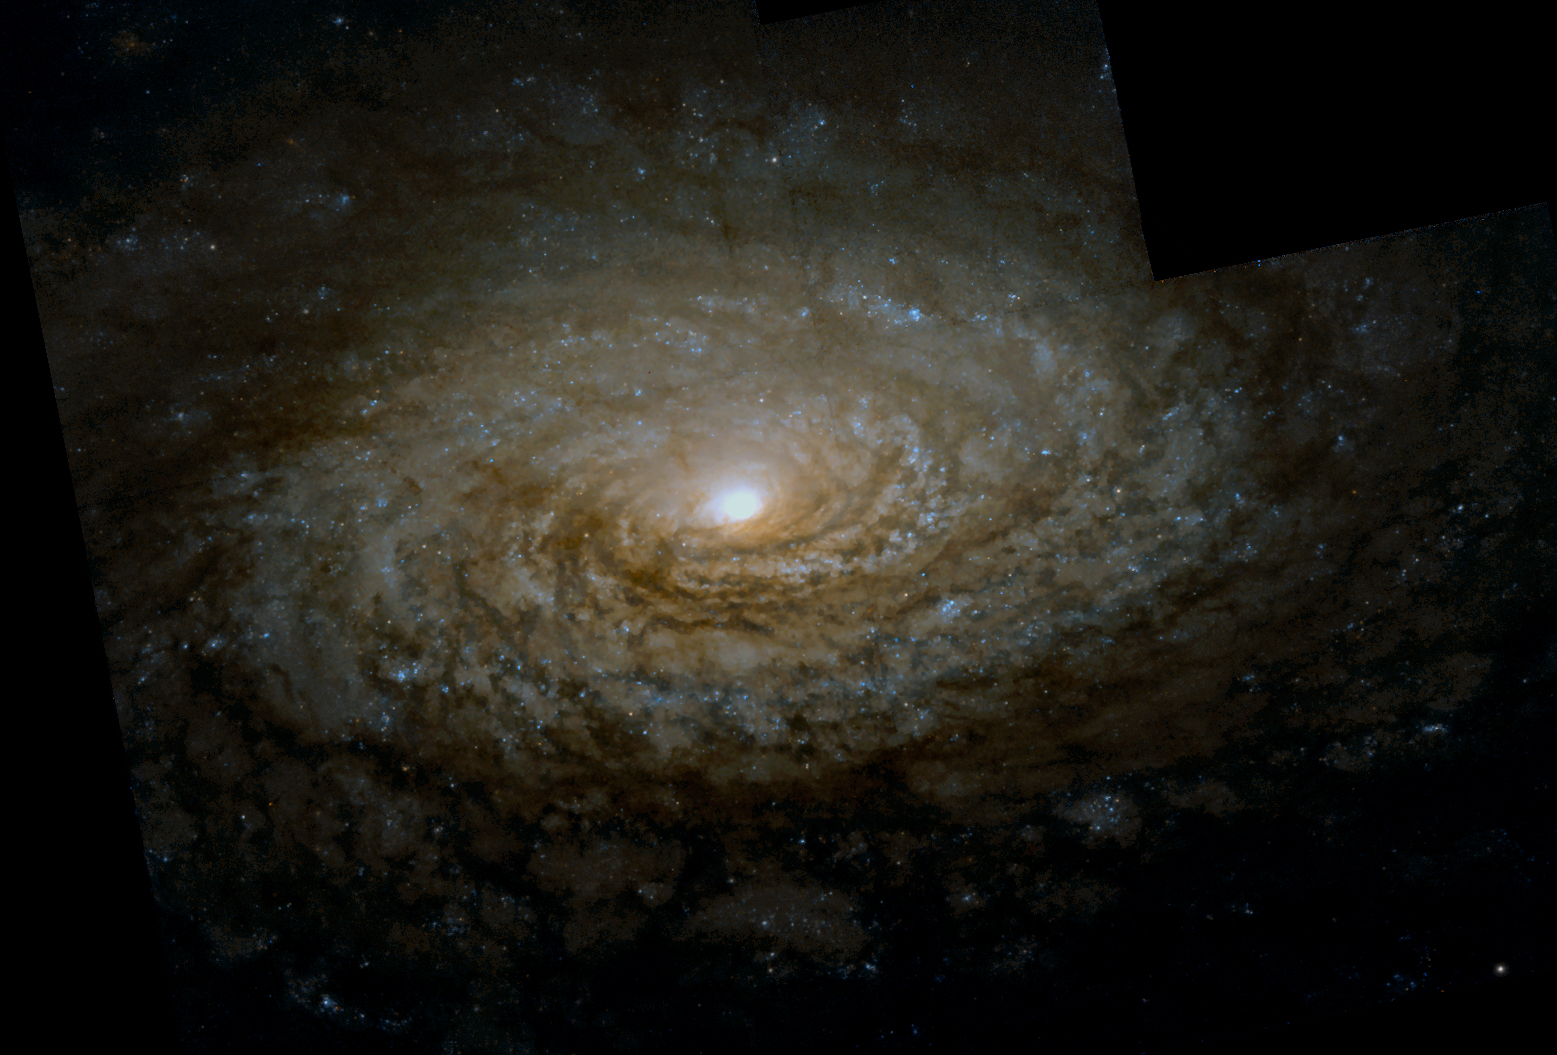
\includegraphics{figures/M63_NGC_5055.jpg}}
\end{center}

\begin{flushright}
{ \tiny \em -- HST/STScI/NASA }
\end{flushright}

\vfill
\end{slide}


%------------------------------------------------------------------------------
\begin{slide}
\begin{center}
{\large \color{red} 
                  NGC 1300 (Sb)  }
\end{center}

\begin{center}
\vskip -0.0in
\scalebox{0.25}{\hskip 0.0in 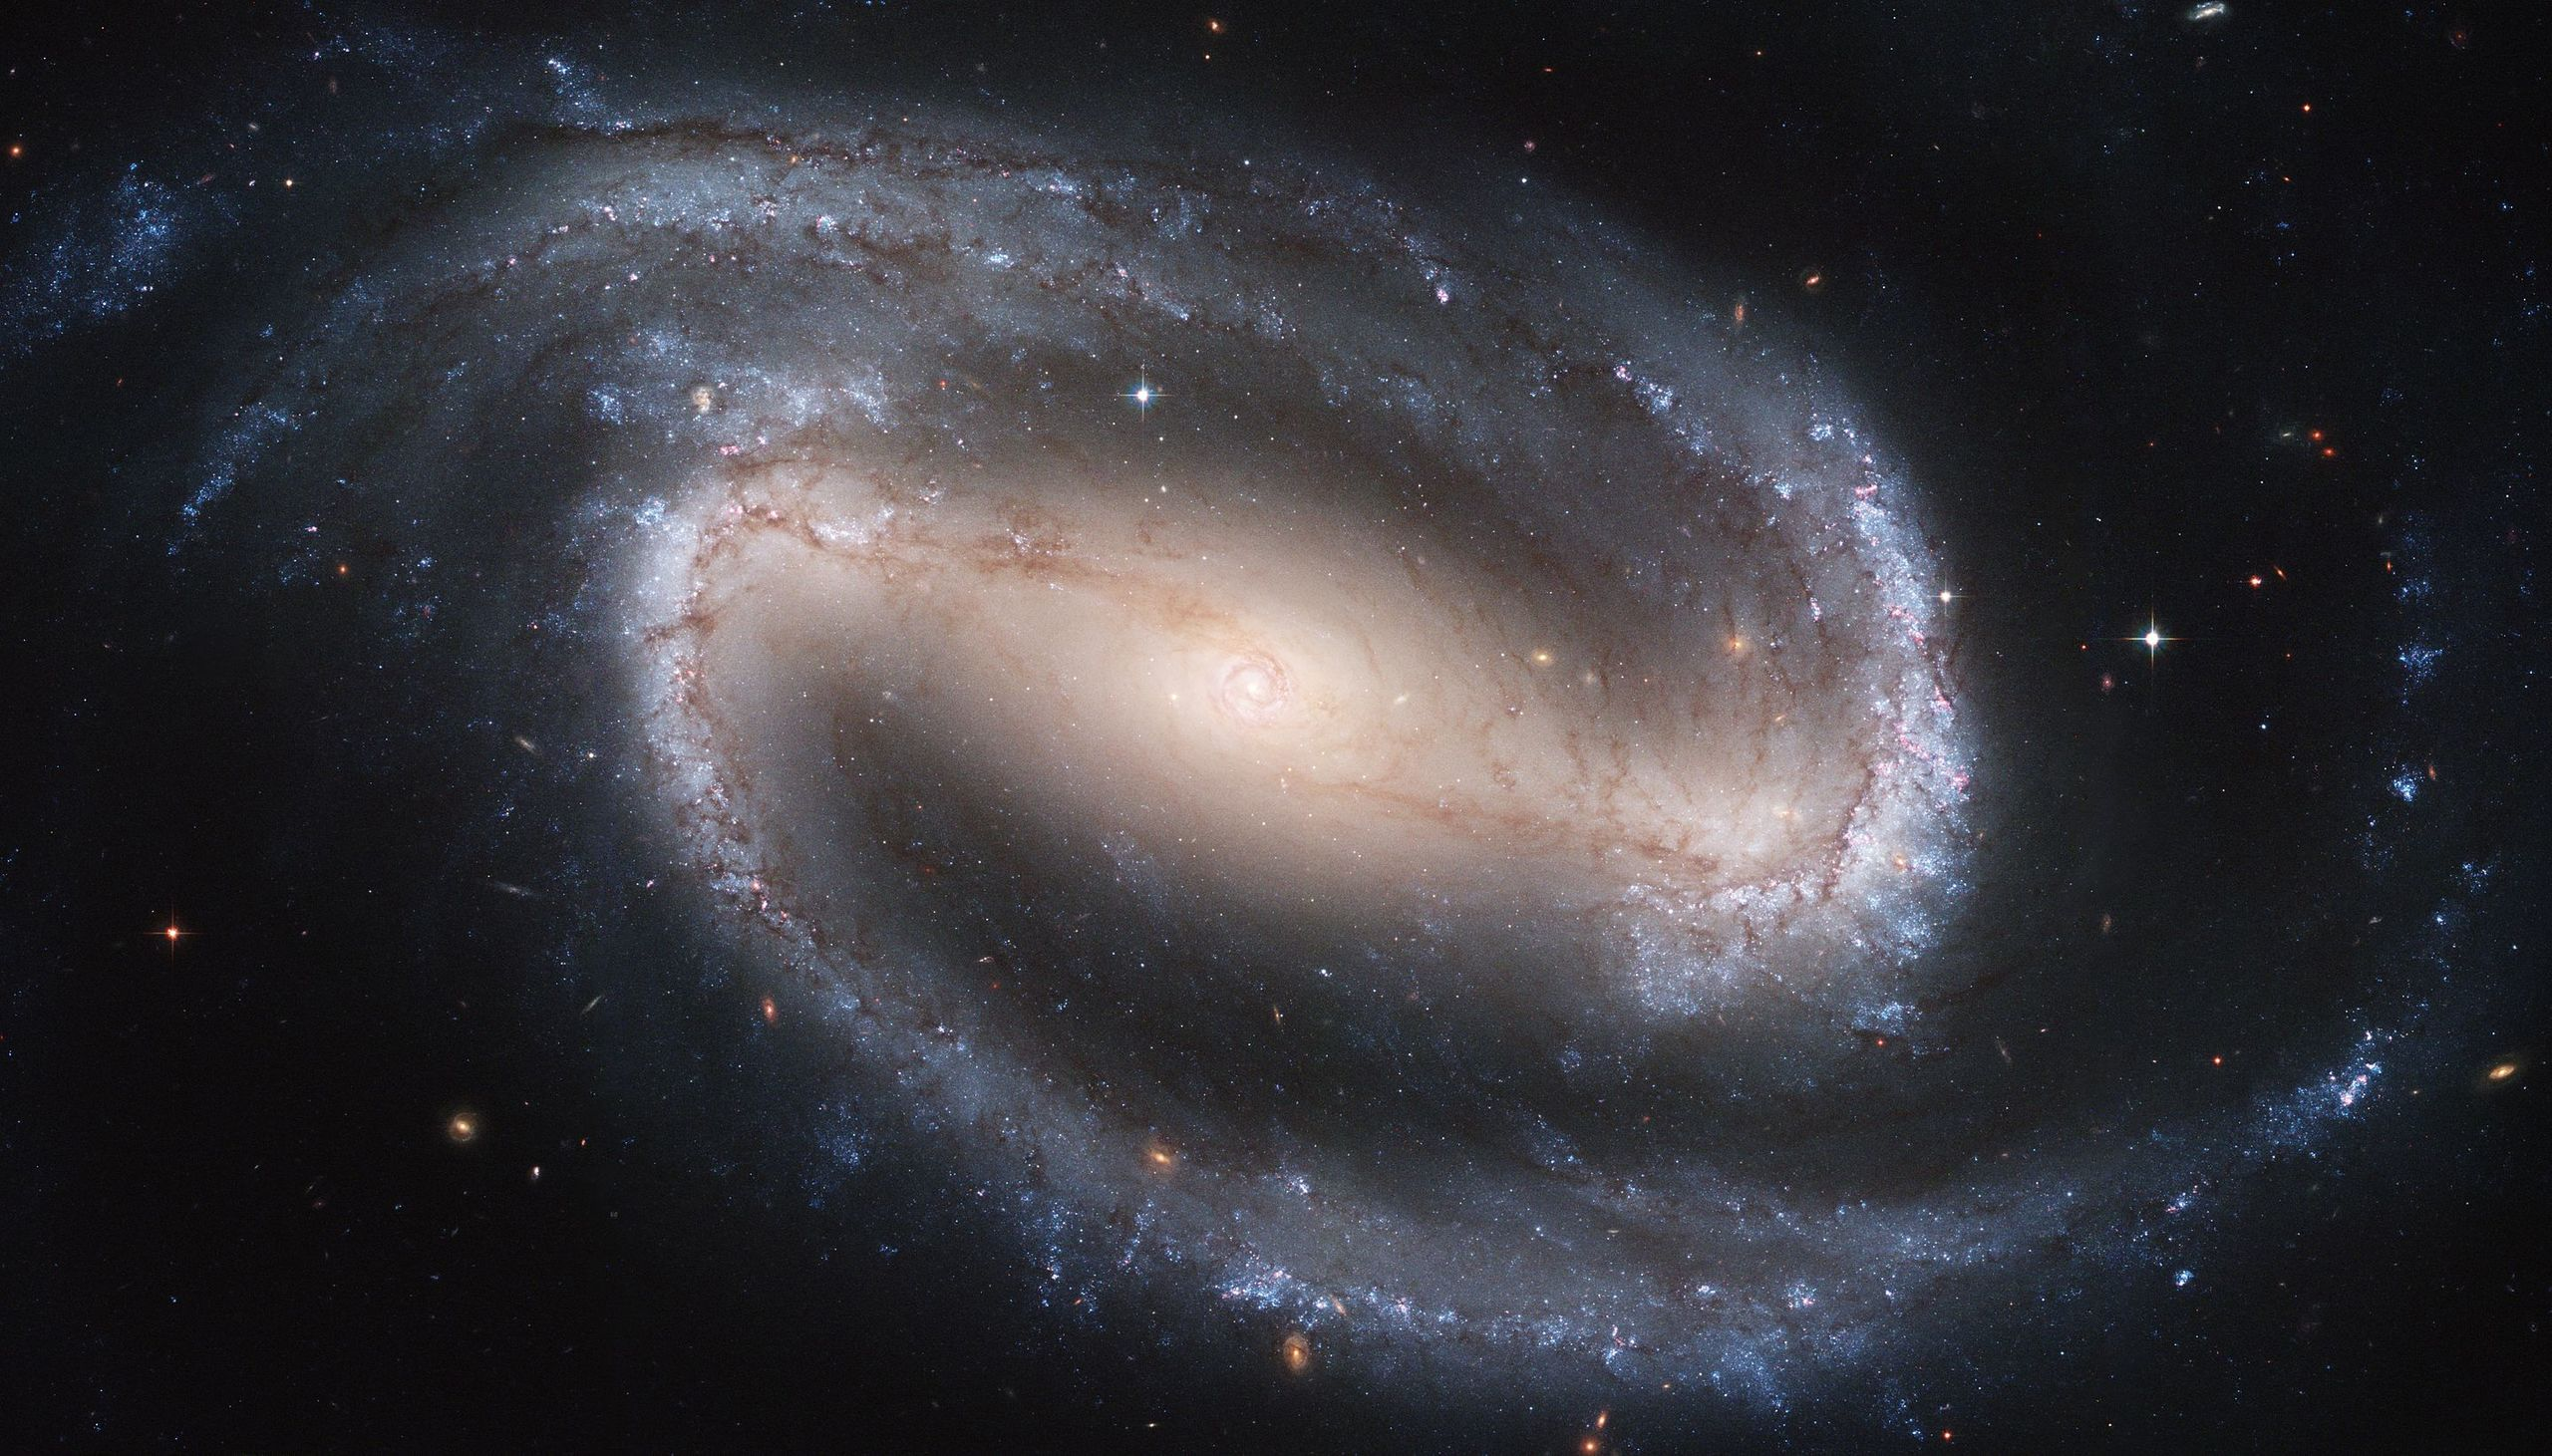
\includegraphics{figures/Hubble2005-01-barred-spiral-galaxy-NGC1300}}
\end{center}

\begin{flushright}
{ \tiny \em -- HST/STScI/NASA }
\end{flushright}

\vfill
\end{slide}


%------------------------------------------------------------------------------
\begin{slide}
\begin{center}
{\large \color{red} 
                  NGC 6745 (Irregular)  }
\end{center}

\begin{center}
\vskip -0.0in
\scalebox{0.8}{\hskip 0.0in 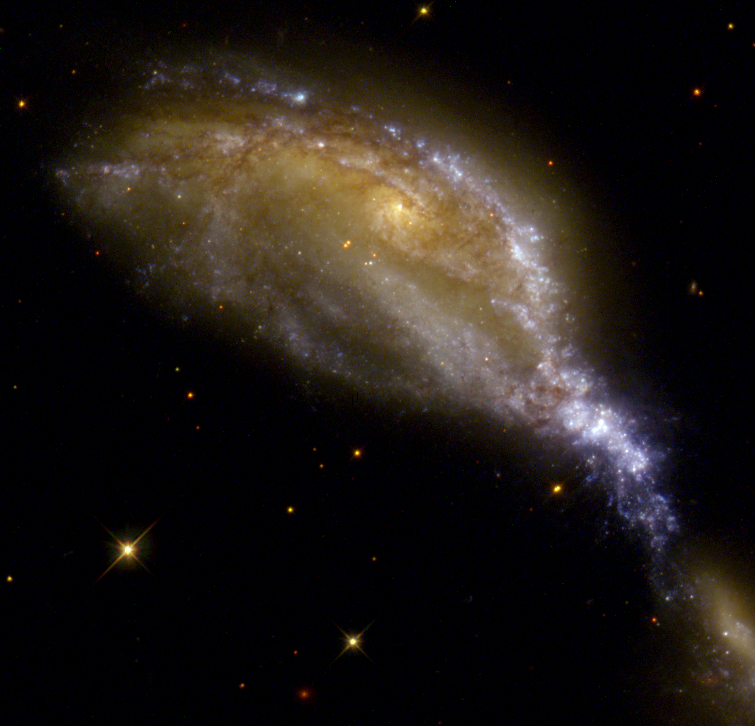
\includegraphics{figures/NGC_6745}}
\end{center}

\begin{flushright}
{ \tiny \em -- HST/STScI/NASA }
\end{flushright}

\vfill
\end{slide}


%------------------------------------------------------------------------------
\begin{slide}
\begin{center}
{\large \color{red} 
                  Grand-Design Spirals (M100, M51, M81, ...)  }
\end{center}

\begin{itemize}
\item Example: M100. Observed features: two major {\bf spiral arms}, each of which can be traced nearly a full revolution. Thin dark
stripes are {\em dust lanes}, that generally follow the spiral arms.
\item This is an example of a {\bf grand-design spiral} galaxy. {\bf Their defining 
features are long, continous, symmetric, spiral arms}. Presumably,
they have been formed by some large-scale process that involves the whole
galaxy. Grand design spirals almost always have two main arms (two-fold symmetry). 
\item Note: grand-design spirals are actually {\em a minority} of all spiral
galaxies ($\sim 10\%$); they are, however, very overrepresented in textbooks.
\end{itemize}

\vfill
\end{slide}


%------------------------------------------------------------------------------
\begin{slide}
\begin{center}
{\large \color{red} 
                  Intermediate-scale Spirals (M101, M33, MW, ...)  }
\end{center}

\begin{itemize}
\item Example: M101. Spiral arms still prominent and well-defined, but less
regular than in grand design spirals. Arms can be traced by $\sim$half a
revolution. Prominent dust lanes still present, with bright ``knots'' of
star formation along the spiral arms.

\item This is an example of {\bf intermediate-scale spiral} structure.
{\bf The defining property is spiral structure that's still coherent over
scales comparable to the galaxy size, but not over the whole galaxy}. In
contrast to grand-design spirals, these don't give an impresson of being
long lived.

\item Another example: M33. The arms are less regular than in M101, but
still satisfies the criteria for an intermediate-scale spiral. One of the
nearest spiral galaxies.
\end{itemize}

\vfill
\end{slide}


%------------------------------------------------------------------------------
\begin{slide}
\begin{center}
{\large \color{red} 
                  Flocculent (fluffy) spirals (M63, NGC 4414, ...)  }
\end{center}

\begin{itemize}
\item Example: M63. Each spiral arm can be followed over only a small angle
and the overall spiral pattern is composed of many patchy arms segments.

\item This is an example of a {\bf flocculent spiral galaxy}.
{\bf Their spiral structure is locallized, with many short, poorly defined,
arms.}

\item In galaxies like these, there's probably no (or very little) causal
connection between the arms on the opposite sides of the galaxy. Their
origin is likely to be {\em local}, rather than global.

\item Note: the classification of spiral arms is independent of the Huble
type. E.g., both M51 and M63 are classified as Sbc, though they
significantly differ in appearance (Elmegreen \& Elmegreen 1987)

\end{itemize}

\vfill
\end{slide}


%------------------------------------------------------------------------------
\begin{slide}
\begin{center}
{\large \color{red} 
                  Galaxies with bars (NGC 1300, NGC 1073, ...)  }
\end{center}

\begin{itemize}
\item Example: NGC 1300. The most striking feature is the {\bf bar},
spanning almost the diameter of the galaxy. Two spiral arms are very
symmetrical. They can be followed almost for a full circle (on deep images).
This particular galaxy is a {\em grand-design spiral}.

\item Note that there are sharp, straight, dust lanes spanning the length of
the bar. The spiral arms start at the tips of the bar. At the start of each
spiral arm, there is a cluster of HII regions (i.e., rapid star formation is
occuring). {\bf These are all common features in barred spiral galaxies.}

\end{itemize}

\vfill
\end{slide}


%------------------------------------------------------------------------------
\begin{slide}
\begin{center}
{\large \color{red} 
                  Irregulars (NGC 6745, ...)  }
\end{center}

\begin{itemize}
\item In the framework of Hubble classification, an {\em irregular} galaxy
is a bit of a catch-all bin for anything that doesn't fit. In some cases we
can still guess what is going on.

\item Example: NGC 6745. This galaxy is lopsided and warped, exhibiting a
tail of young, blue stars to the lower right. That said, the main body still
shows some semblance of spiral structure.

\item These features are likely a result of a recent encounter with a
smaller galaxy (hiding in the bottom right). The tides inflicted by the
small galaxy have compressed and shocked the ISM in NGC 6745, leading to a
burst of star formation (including in the tail of stars pointing toward the
``intruder'').

\end{itemize}

\vfill
\end{slide}


%------------------------------------------------------------------------------
\begin{slide}
\begin{center}
{\large \color{red} 
                  Star formation in spiral arms  }
\end{center}

\begin{itemize}
\item In all the examples we've looked so far, the light in spirals is
dominated by luminous, young, stars and HII regions.

\item These massive stars typically live less than $\sim 10$Myr (compared to
typical orbital periods of $\sim 100$Myr); i.e., they we can't be observing
them far from where they were created.

\item Therefore, {\bf the star-formation rate (SFR) in the spiral arms must
be much higher than in the rest of the disk}.

\item {\color{blue} This brings up an interesting question: {\bf are spiral arms just areas of
increased star formation} (as opposed to increase of overall stellar number
density)?}

\end{itemize}

\vfill
\end{slide}

%------------------------------------------------------------------------------
\begin{slide}
\begin{center}
{\large \color{red} 
                  Multi-wavelength Observations of Spiral Arms  }
\end{center}

\begin{itemize}
\item Multi-wavelength observations give us further insight into the nature
of spiral structure.

\item {\bf Visible} (blue) light is {\bf dominated by young stars}, and it
traces {\bf star formation}.  {\bf Near-IR} light is {\bf dominated by older
populations} (giants), and it's a tracer of {\bf mass}.

\item Let's take a look...

\end{itemize}

\vfill
\end{slide}


%------------------------------------------------------------------------------
\begin{slide}

\begin{center}
{\large \color{red} 
                  M51 in the Visible and Near-IR  }
\end{center}

\begin{center}
\vskip -0.0in
\scalebox{0.85}{\hskip 0.0in 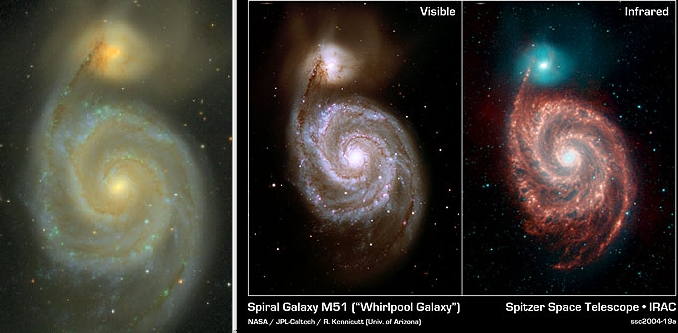
\includegraphics{figures/M51_comp}}
\end{center}

\begin{flushright}
{ \tiny \em -- Spitzer/JPL Caltech/NASA }
\end{flushright}

\end{slide}


%------------------------------------------------------------------------------
\begin{slide}

\begin{center}
\vskip -0.0in
\scalebox{0.85}{\hskip 0.0in 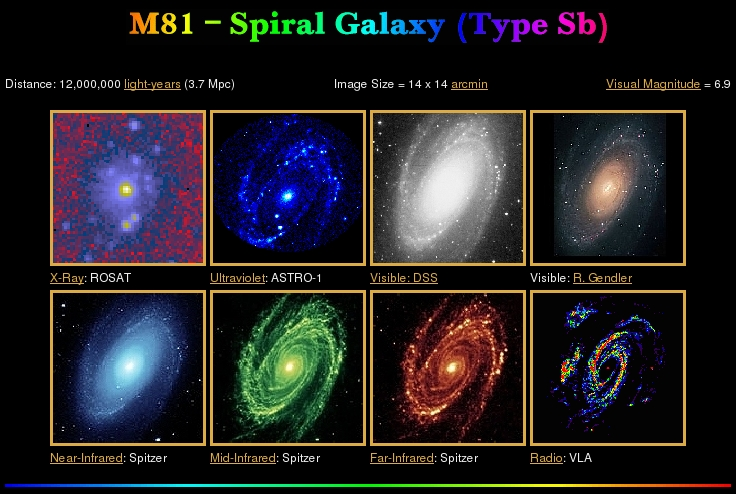
\includegraphics{figures/M81_multiLambda}}
\end{center}

\begin{flushright}
{ \tiny \em -- Spitzer/IPAC/NASA }
\end{flushright}

\end{slide}


%------------------------------------------------------------------------------
\begin{slide}
\begin{center}
{\large \color{red} 
                  Multi-wavelength Observations of Spiral Arms  }
\end{center}

\begin{itemize}

\item We find that {\bf nearly all grand-design spirals are detectable in
the near-IR} (e.g., Eskridge et al.  2002) as are galaxies with
intermediate-scale spiral structure.

\item This leads us to conclude that {\bf the spiral pattern exists both in
the surface density -- the mass -- as well as the star formation rate}. 
This is the strongest piece of evidence that spiral structure is a {\bf
density wave}.

\item Also: Typically, the arm traced by the young stars is displaced
slightly inside the old-star arm.

\end{itemize}

\vfill
\end{slide}


%------------------------------------------------------------------------------
\begin{slide}
\begin{center}
{\large \color{red} 
                  Floculent Spirals: Sheared patches of SFR  }
\end{center}

\begin{itemize}

\item What about floculent spirals? They do not exhibit equally noticable spiral structure in near-IR.

\item This strongly points to their structure more likely to be {\bf due to a local process}.
The observations are consistent with {\bf the floculent spiral
structure arising due to patches of star formation, that have been sheared into a 
spiral on timescales comparable to lifetimes of
the young stars} (Elmegreen \& Elmegreen 1984; Thornley 1996).

\item This would imply these spirals are {\bf transient}, surviving on timescales of $\sim 10$Myr.

\item These perturbations do not change the overall mass distribution within the disk of the galaxy.

\end{itemize}

\vfill
\end{slide}


%------------------------------------------------------------------------------
\begin{slide}
\begin{center}
{\large \color{red} 
                  Spiral Structure with Other Tracers  }
\end{center}

\begin{itemize}
\item {\bf Relativistic electrons} trace the spirals (inside the bright-star arm)
\item {\bf Molecular gas} (CO) traces the gas/dust arm
\item {\bf Neutral atomic gas} coincides with the spiral arms
\item {\bf HII regions} trace the bright-star spiral arms
\end{itemize}

Important observation: it's an observational fact that {\bf spiral structure
is present only in galaxies where there's gas}. So even though we see the spiral
structure in overall (old-star) stellar density, {\bf gas is somehow required
for it to persist}.

\vfill
\end{slide}


%------------------------------------------------------------------------------
\begin{slide}
\begin{center}
\vskip 3in
{\large \color{red} Quantifying Spiral Structure  }
\end{center}

\end{slide}

%------------------------------------------------------------------------------
\begin{slide}
\begin{center}
{\large \color{red} 
                  The Geometry of Spiral Structure  }
\end{center}

\begin{center}
\vskip -0.0in
\scalebox{0.66}{\hskip 0.0in 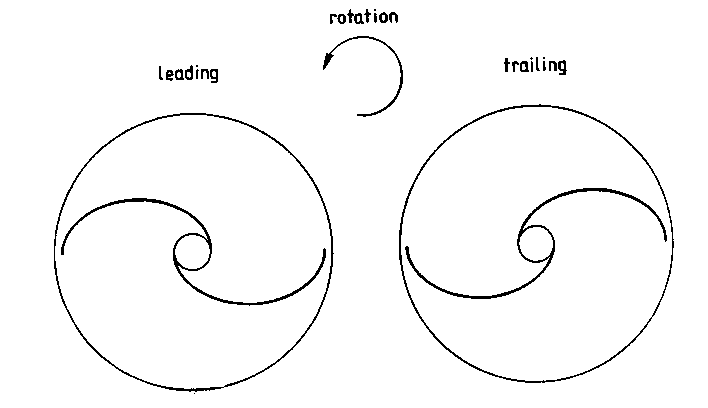
\includegraphics{figures/lead_trail.png}}
\end{center}

Definitions: an arm is {\bf leading} if its outer tip points in the direction of
rotation, and {\bf trailing} otherwise.

It's not easy to tell a leading from a trailing arm; it's degenerate with
galaxy inclination (see BT Fig 6.5). It's possible to break the degeneracy
by observing dust-induced dimming; these kinds of observations reveal
{\bf nearly all spiral arms are trailing}.

\vfill
\end{slide}


%------------------------------------------------------------------------------
\begin{slide}
\begin{center}
{\large \color{red} 
                 Characterization of Spiral Structure  }
\end{center}
\begin{itemize}
\item The measures of symmetry ($m$) and amplitude ($A_m$) of spiral structure:
\eq{
	\frac{I(R,\phi)}{\bar{I}(R)} = 1 + \sum_{m=1}^\infty A_m(R)cos m[\phi - \phi_m(R)]; \mspace A_m(R) > 0
}
where $\bar{I}(R)$ is the azimuthally averaged surface brightness at radius $R$ and
$A_m$ and $\phi_m$ are the amplitude and phase of the $m$th Fourier component. If
a particular mode $m$ strongly dominates, the spiral is said to have $m$-fold
rotational symmetry; $m$ is {\bf the number of arms}.

\item If a single Fourier component $m$ dominates, the {\bf strength} of the
spiral can be quantified as the arm-interarm surface-brightness ratio:
\eq{
	K = \frac{1 + A_m}{1 - A_m}
}

\end{itemize}
\vfill
\end{slide}

%------------------------------------------------------------------------------
\begin{slide}
\begin{center}
{\large \color{red} 
                  The Symmetry of Spiral Structure  }
\end{center}

\begin{center}
\vskip -0.0in
\scalebox{0.8}{\hskip 0.0in 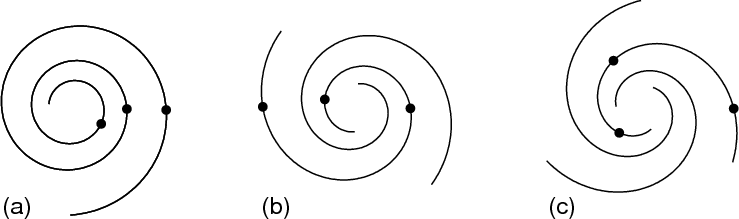
\includegraphics{figures/densitywaves-img127.png}}
\end{center}

Density waves with $m=1$, $m=2$ and $m=3$ symmetry. Reproduced from Griv \& Gedalin
(2010).

\vfill
\end{slide}

%------------------------------------------------------------------------------
\begin{slide}
\begin{center}
{\large \color{red} 
                 Characterization of Spiral Structure  }
\end{center}
\begin{itemize}

\item The {\bf pitch angle}, $\alpha$, at any radius is the angle between the tangent to the arm,
and the circle $R = constant$; by definition, $0 < \alpha < 90^\circ$.

Related to the pitch angle is the {\bf shape function} of a spiral wave:
\eq{
	m \phi + f(R, t) = {\rm constant} \mspace {\rm (mod}\, 2\pi {\rm)}
}
in a galaxy with $m$-fold symmetry. The pitch angle is then given by {\color{blue} $\cot \alpha = |R \p \phi / \p R|$}.

\item It's also useful to introduce the {\bf radial wavenumber}, $k$,
\eq{
	k(R, t) \equiv \frac{\p f(R, t)}{\p R}
}
Note that the sign of $k$ determines whether the arms are leading ($k < 0$) or
trailing ($k > 0$). With this definition, the pich angle is {\color{blue} $\cot \alpha = |k R / m|$}.

\end{itemize}
\vfill
\end{slide}


%------------------------------------------------------------------------------
\begin{slide}
\begin{center}
{\large \color{red} 
                 Characteristic Scales (Observational Facts) }
\end{center}
\begin{itemize}

\item In grand-design spirals, we find $\bm{0.15 \lesssim A_2 \lesssim 0.6}$ (Rix \& Zaritsky 1995),
\item This corresponds to arm-interarm ratios of $\bm{1.4 \lesssim K \lesssim 4}$;
\item In most grand-design spirals {\bf $m=2$ mode dominates} (though some show $m=3$). $m=2$ domination
is an observational fact requiring a theoretical explanation;
\item Significant fraction of galaxies is lopsided in the outer parts $\bm{A_1 \gtrsim 0.2}$ (Rix \& Zaritsky 1995);
\item Large majority of arms are {\bf trailing}, and
\item Characteristic pitch angles are in $\bm{10^\circ \lesssim \alpha \lesssim 15^\circ}$ range.

\end{itemize}
\vfill
\end{slide}


%------------------------------------------------------------------------------
\begin{slide}
\begin{center}
{\large \color{red} 
                 The Winding Problem }
\end{center}

Let's conduct a thought experiment where we start a spiral arm that is a
straight line at $t = 0$, and that rotates together with the disk:
\eq{
	\phi(R, t) = \phi_0 + \Omega(R) t
}
I.e., you can imagine we've ``drawn'' a line of O stars embedded in an otherwise
FGKM-dominated disk. We let these revolve around the center.

The pitch angle will then evolve as:
\eq{
	\cot \alpha = R t | \frac{d \Omega}{d R} |
}
Taking a galaxy with a flat circular-speed curve, $R\Omega(R) = v_c = 200 {\rm km/s}$,
at $R = 5$kpc and $t = 10$Gyr, we find $\alpha = 0.14^\circ$, {\em far smaller
than the observed pitch angles of $\sim 10^\circ-15^\circ$}. This is the {\bf
winding problem} (Linblad 1925).

\vfill
\end{slide}

%------------------------------------------------------------------------------
\begin{slide}

\begin{center}
{\large \color{red} 
                 The Winding Problem }
\end{center}

\begin{center}
\vskip -0.0in
\scalebox{1}{\hskip 0.0in 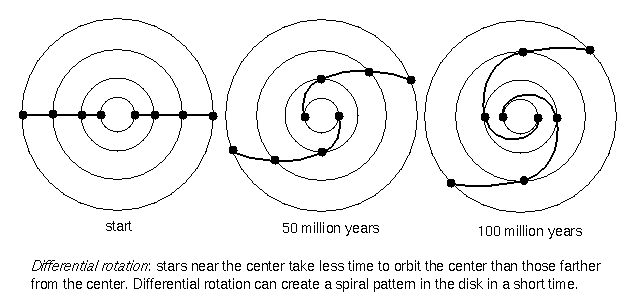
\includegraphics{figures/Wproblem1}}
\end{center}

\vfill
\end{slide}


%------------------------------------------------------------------------------
\begin{slide}

\begin{center}
{\large \color{red} 
                 The Winding Problem }
\end{center}

\begin{center}
\vskip -0.0in
\scalebox{1}{\hskip 0.0in 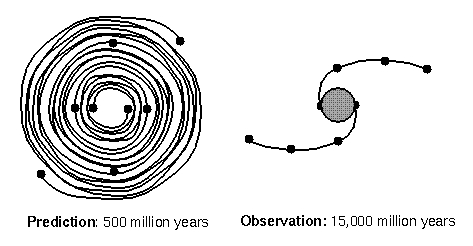
\includegraphics{figures/Wproblem2}}
\end{center}

The Winding Problem: most spiral galaxies would be tightly wound by
now, which is inconsistent with observations.

Implication: Spiral arms {\bf cannot be a static structure} (i.e. {\bf at 
different times, arms must be made of different stars}). If that's so,
what are they?

\vfill
\end{slide}


%------------------------------------------------------------------------------
\begin{slide}
\begin{center}
\vskip 3in
{\large \color{red} Theories of Spiral Structure  }
\end{center}

\end{slide}

%------------------------------------------------------------------------------
\begin{slide}

\begin{center}
{\large \color{red} 
                 Theories of Spiral Structure }
\end{center}

Despite 50 years of work, spirals are not fully understood. It
seems clear now that the spiral structure of galaxies is a complex
problem where details do not have a unique or tidy answer.

Differential rotation clearly plays a central role, as well as global
instabilities, stochastic spirals, and the shocks patterns that can
arise in shearing gas disks when forced by bars.

Despite that, the general picture is reasonably clear: the grand
design and intermediate-scale spirals are explained by {\bf density
waves in stellar density and potential} (either stationary or 
transient, e.g., perhaps from a recent close encounter with a nearby
galaxy), while {\bf flocculent spirals arise due to shearing of
localized patches of star formation}.

\vfill
\end{slide}


%------------------------------------------------------------------------------
\begin{slide}

\begin{center}
\vskip -0.4in
\scalebox{0.66}{\hskip 0.0in 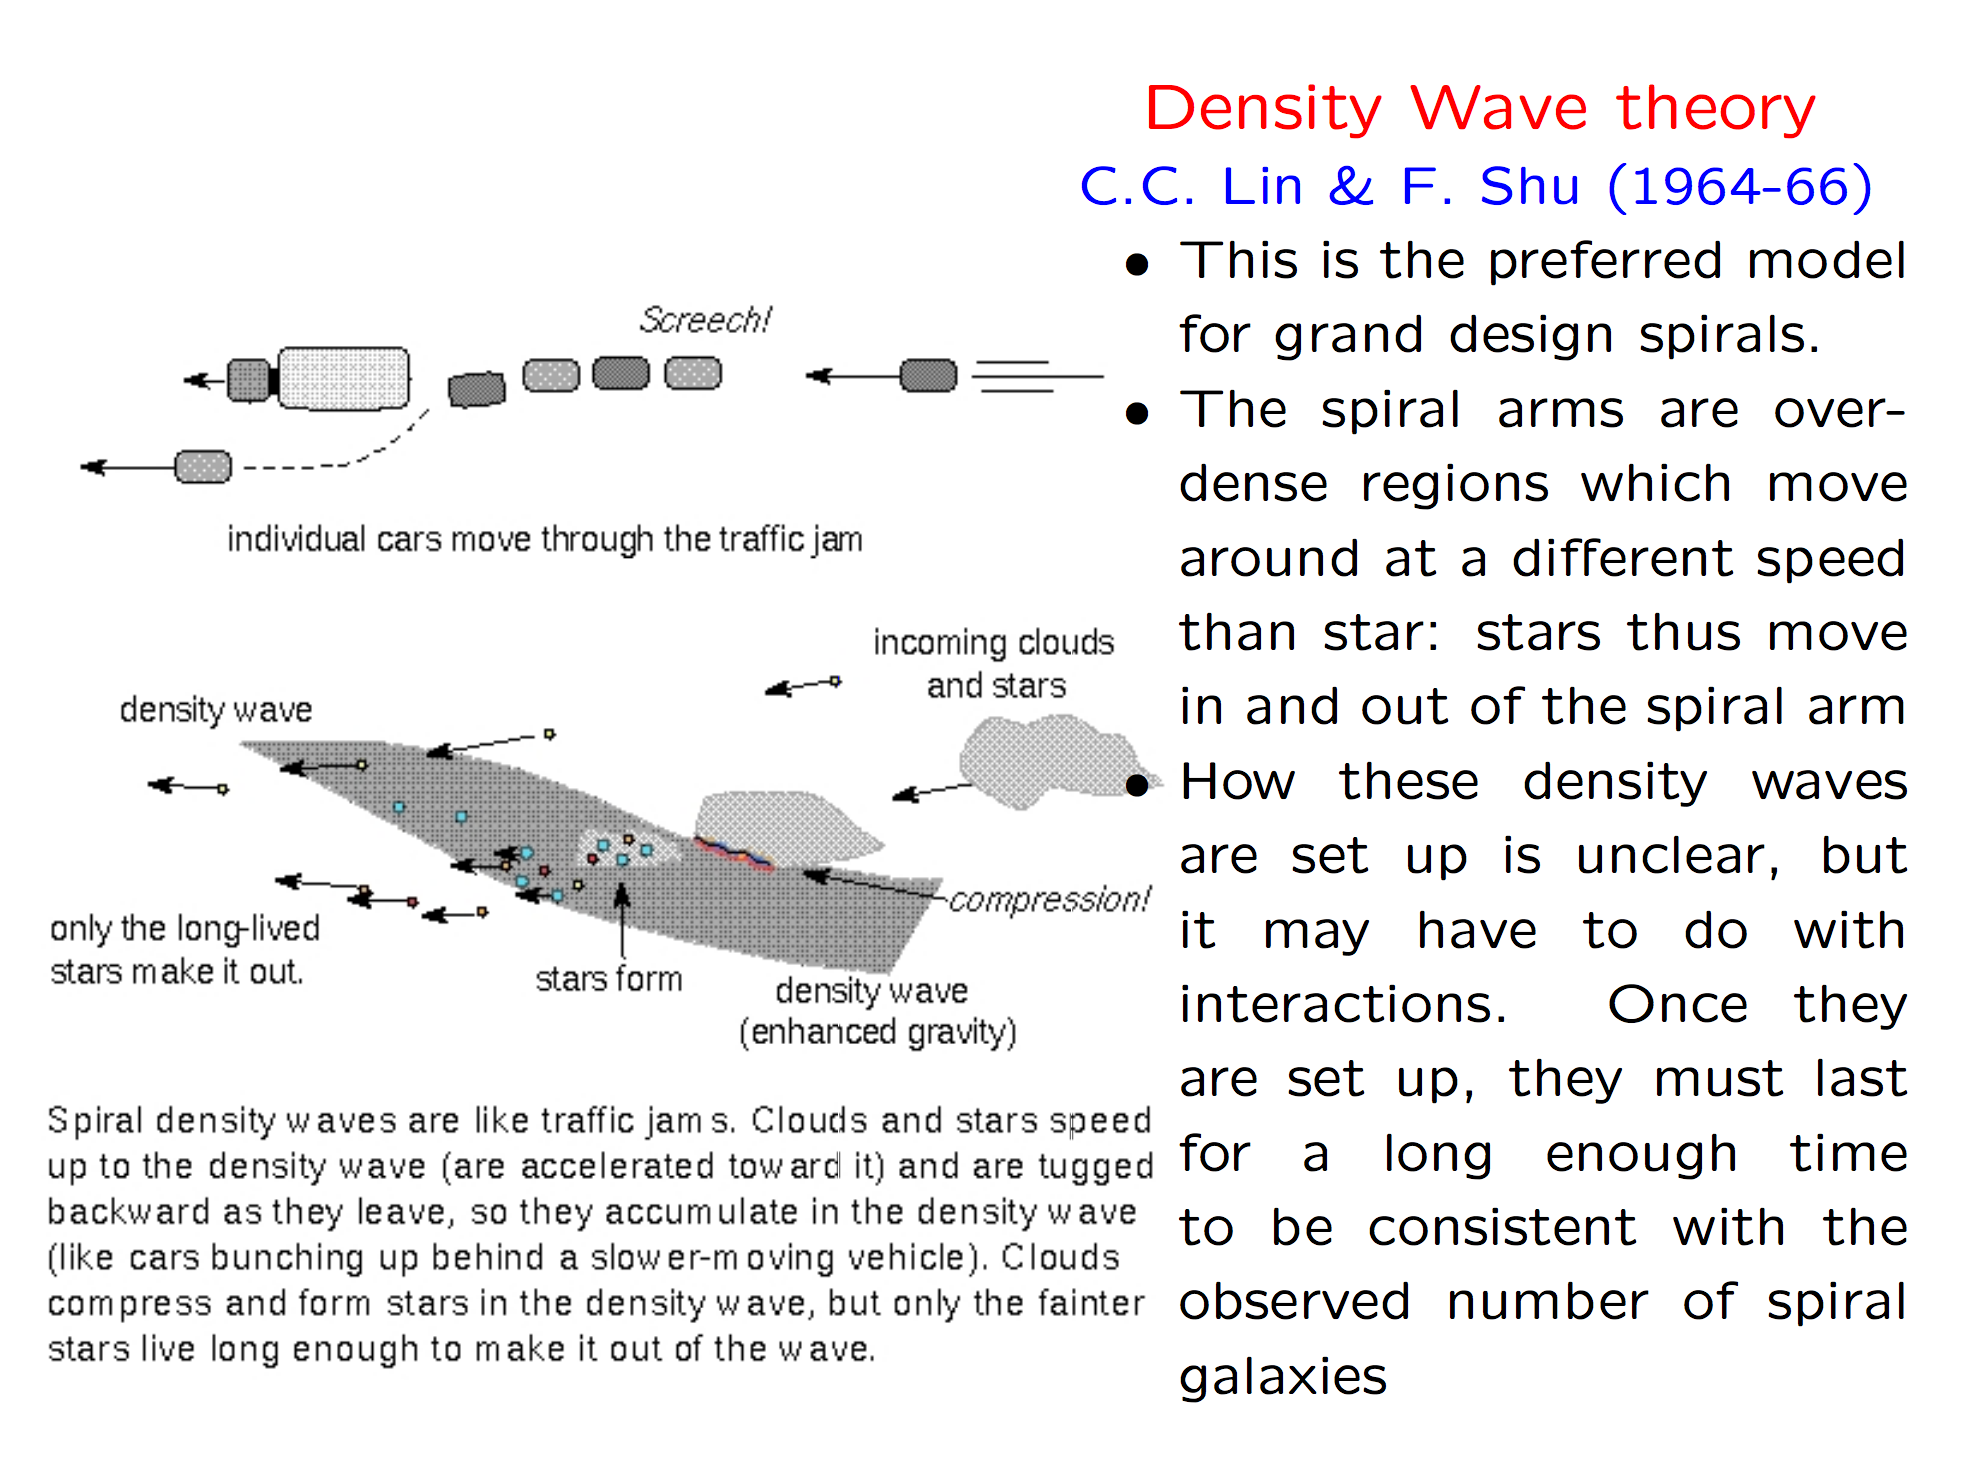
\includegraphics{figures/density-wave-slide.png}}
\end{center}

\end{slide}

%------------------------------------------------------------------------------
\begin{slide}

\begin{center}
{\large \color{red} 
                 Stochastic Self-Propagating Star Formation }
\end{center}

\begin{center}
\scalebox{1}{\hskip 0.0in 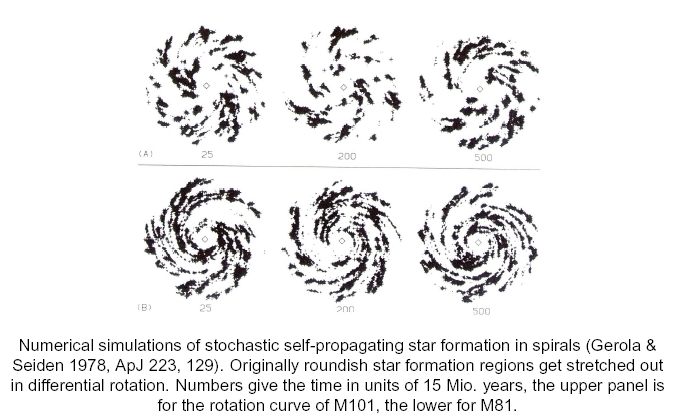
\includegraphics{figures/stoch}}
\end{center}

\end{slide}


%------------------------------------------------------------------------------
\begin{slide}

\begin{center}
{\large \color{red} 
                 Understanding Density Wave Theory }
\end{center}

Let's develop a better understanding of how density waves come about:

\begin{itemize}
\item Let's observe a galaxy from a rotating coordinate system which 
revolves at some speed, say $\Omega_p$. {\em (we'll later identify this with
the pattern speed of the spiral arms.)}

\item For an axisymmetric disk with a flat rotation curve (a good
first order approximation to the disk of a spiral galaxy), this
rotation speed will match up with the rotation speed at some
radius $R$. This is the {\color{blue} corotation radius} for pattern
speed $\Omega_p$.

\item Particles inside this
radius will appear to revolve in the direction of the frame rotation (prograde).
Outside this corotation radius, they will be retrograde.

\end{itemize}

\vfill
\end{slide}

%------------------------------------------------------------------------------
\begin{slide}

\begin{center}
{\large \color{red} 
                 Understanding Density Wave Theory }
\end{center}

Given $\Omega_p$, at some radii open orbits become closed: for a
star which completes two radial oscillations while performing
one complete azimuthal trip in the rotating frame, we get
elliptical orbits with the center at the center of the potential
(so called 2/1 orbits). Similarly, a ratio of 3/2 gives a three-armed
cloverleaf pattern, etc.

\begin{center}
\vskip -0.45in
\scalebox{0.9}{\hskip 0.0in 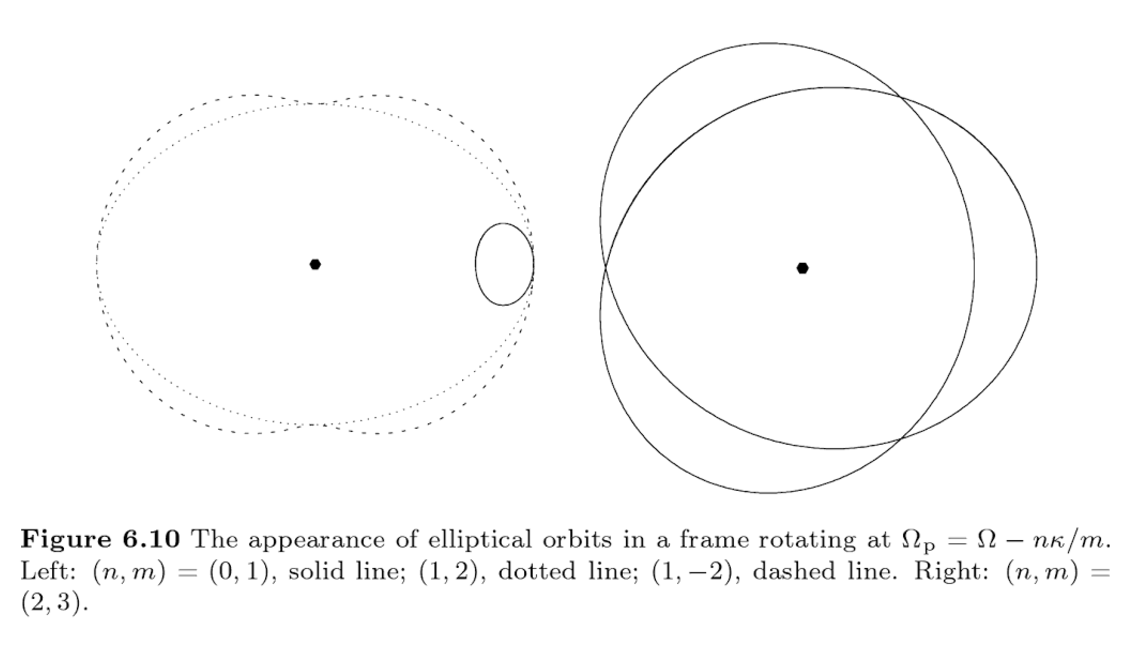
\includegraphics{figures/BT-fig6_10.png}}
\end{center}

\vfill
\end{slide}

%------------------------------------------------------------------------------
\begin{slide}

\begin{center}
{\large \color{red} 
                 Kinematic Density Waves }
\end{center}

These figures appear at every radius, if they're cleverly oriented, they can
{\bf generate spiral- and bar-like patterns}:

\begin{center}
\scalebox{1.0}{\hskip 0.0in 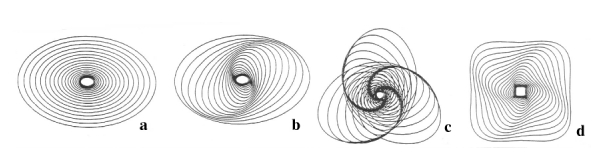
\includegraphics{figures/orbits}}
\end{center}

{\bf a)} a bar can be produced by aligning a series of concentric elliptical orbits
{\bf b)} if each ellipse is given an azimuthal offset proportional to $\sqrt{R}$, the effect is a two-armed spiral
{\bf c)} a set of 3/2 orbits produces a three armed spiral
{\bf d)} a set of 4/1 orbits produces a four armed pattern

\end{slide}


%------------------------------------------------------------------------------
\begin{slide}

\begin{center}
{\large \color{red} 
                 Kinematic density waves }
\end{center}

\begin{itemize}

\item The above result shows how we can set up arrangements of orbits
in a disk galaxy that results in bar- or spiral-like {\bf density waves}.
We call these {\bf kinematic} because they only involve
the kinematics of orbits in an axisymmetric potential.

\item When the majority of the stars are arranged in these patterns,
the mass asymmetry will begin to affect the
overall potential. The stars will begin to deviate from these orbits.

\item A {\bf major goal of spiral-structure theory} is to {\bf determine whether
the non-axisymmetric potential due to to the spiral itself can} ``coordinate''
the orientations and drift rates of orbits in such a way as to {\bf produce
long-lived, self-sustaining, spiral patterns}

\item Question: can perturbations generate/sustain spiral density waves?

\end{itemize}

\vfill
\end{slide}

%------------------------------------------------------------------------------
\begin{slide}

\begin{center}
{\large \color{red} 
                 Stability of Differentially Rotating Disks }
\end{center}

This is not an easy question to answer in general. It's an impossible
one to answer analytically, without resorting to approximations.

One approximation where a solution can be found analytically is one
where the (spiral) density waves are tightly wound (their radial
wavelength is much less than the radius; $\Delta R \ll R$).

When that's the case, the long-range coupling is shown to be negligible,
therefore the response is determined locally, and the relevant solutions
turn out to be analytic.

This is called {\bf tight-winding, short-wavelength, approximation}. It's
also known as the WKB approximation, by analogy with a mathematically
similar procedure in quantum mechanics.

You can follow the details in Binney \& Tremaine, \S 6; here, we will
only confine ourselves to final results and qualitative comments.

\end{slide}

%------------------------------------------------------------------------------
\begin{slide}

\begin{center}
{\large \color{red} 
                 Stability of Differentially Rotating Disks }
\end{center}

BT show how to derive the dispersion relation for {\bf spiral density
waves in gaseous disks} (i.e., disks possessing an equation of state)
in the tight-winding limit:
\eq{
	(m\Omega - \omega)^2 = \kappa^2 - 2\pi G \Sigma |k| + k^2 v_s^2
}.

An {\bf analogous relation for stellar disks is}:
\eq{
	(m\Omega - \omega)^2 = \kappa^2 - 2\pi G \Sigma |k| F[(m \Omega - \omega)/\kappa, k \sigma_R / \kappa]
}
where function $F$ is defined in BT (eq.6-63).

\end{slide}

%------------------------------------------------------------------------------
\begin{slide}

\begin{center}
{\large \color{red} 
                 Stability of Differentially Rotating Disks }
\end{center}

What does this mean? Remember that the dispersion relation tells us about the response of
a system to plane wave perturbations of the form:
\eq{
	\Sigma(R, \phi, t) \propto e^{i[m \phi + f(R, t)]}
}
For a given wavenumber $k$, $\omega$ is {\bf the frequency at which the plane
wave will oscillate}. However, if $\omega^2 < 1$, the resulting frequency
is {\em imaginary}, ``oscillations'' are exponential, and {\bf the system
unstable to perturbations at that $k$}.

This gives us a way to explore the stability of galactic disks
to density perturbations.

\vfill
\end{slide}

%------------------------------------------------------------------------------
\begin{slide}

\begin{center}
{\large \color{red} 
                 Stability Criterion (Toomre's $Q$) }
\end{center}

Consider an axially symmetric perturbation in a uniformly rotating ($\kappa = 2\Omega$)
gaseous disk ($m = 0$). The dispersion relation reduces to:
\eq{
	\omega^2 = 4 \Omega^2 -2 \pi G \Sigma |k| + k^2 v_s^2
}

This will be unstable if $\omega < 0$. If also $\Omega = 0$ (non-rotating potential), then
disk is unstable if
\eq{
	|k| < k_J \equiv \frac{2\pi G \Sigma}{v_s^2}
}
$k_J$ can be though of as the {\em Jeans wavenumber} for the gaseous sheet; it defines
the wavelength -- the scale -- at which the sheet will fragment and collapse. Note 
how rotation helps to keep disk stable.

\end{slide}

%------------------------------------------------------------------------------
\begin{slide}

\begin{center}
{\large \color{red} 
                 Stability Criterion (Toomre's $Q$) }
\end{center}

The equivalent in stellar disks results in a relation first derived by (Alar) 
Toomre (1964). Toomre’s local stability criterion for stellar disks is:
\eq{
	Q \equiv \frac{\sigma_R \kappa}{3.36 G \Sigma} > 1
}

When $Q > 1$, the stellar disk is resillient to perturbations (it will ``bounce
back''). When $Q < 1$, the disk will collapse and fragment when perturbed.

It's interesting to note that MW disk is marginally stable.

\end{slide}

%------------------------------------------------------------------------------
\begin{slide}

\begin{center}
{\large \color{red} 
                 Toomre's $Q$ }
\end{center}

\begin{center}
\vskip -0.0in
\scalebox{1.1}{\hskip 0.0in 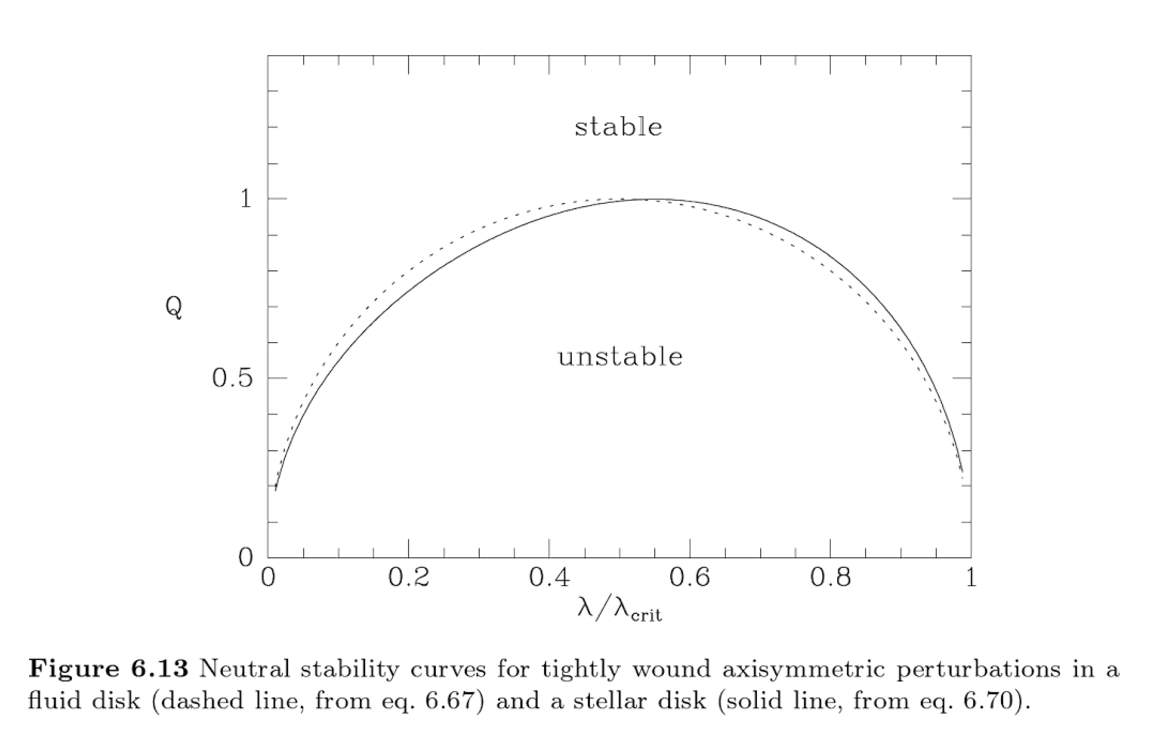
\includegraphics{figures/ToomreQ.png}}
\end{center}

\vfill
\end{slide}

%------------------------------------------------------------------------------
\begin{slide}

\begin{center}
{\large \color{red} 
                 Stability of Differentially Rotating Disks }
\end{center}

What if tight-winding limit is not applicable? There are no analytic
methods -- one must perform numerical experiments (N-body or
other).

These experiments reveal that Toomre's $Q>1$ criterion is a fairly accurate
predictor of stability to axisymmetric modes of all wavelenghts.

But also, they bring some worrisome results, namely that if most of the
kinetic energy of the disk is in rotational motion, then the disk is
usually strongly unstable to large-scale bar-like modes (i.e., the creation
of a bar).

This raises an important questions: why are disk galaxies stable? Ostriker
and Peebles (1973) were the first one ask it, and also point to a solution:
that disks of galaxies are embedded in massive dark-matter halos. Under those
conditions, the disk of a galaxy will be stable as long as $T/|\Phi| < 0.14$
(the {\bf Ostriker-Peebles criterion}).

\vfill
\end{slide}

%------------------------------------------------------------------------------
\begin{slide}

\begin{center}
{\large \color{red} 
                 Bar Instability }
\end{center}

\begin{center}
\vskip -0.0in
\scalebox{0.6}{\hskip 0.0in \includegraphics{figures/bar-instability.png}}
\end{center}

\vfill
\end{slide}

%------------------------------------------------------------------------------
\begin{slide}
\begin{center}
\vskip 3in
{\large \color{red} Barred Galaxies (a very brief overview)  }
\end{center}

\end{slide}

%------------------------------------------------------------------------------
\begin{slide}
\begin{center}
{\large \color{red} 
                  NGC 1300 (Sb)  }
\end{center}

\begin{center}
\vskip -0.0in
\scalebox{0.25}{\hskip 0.0in 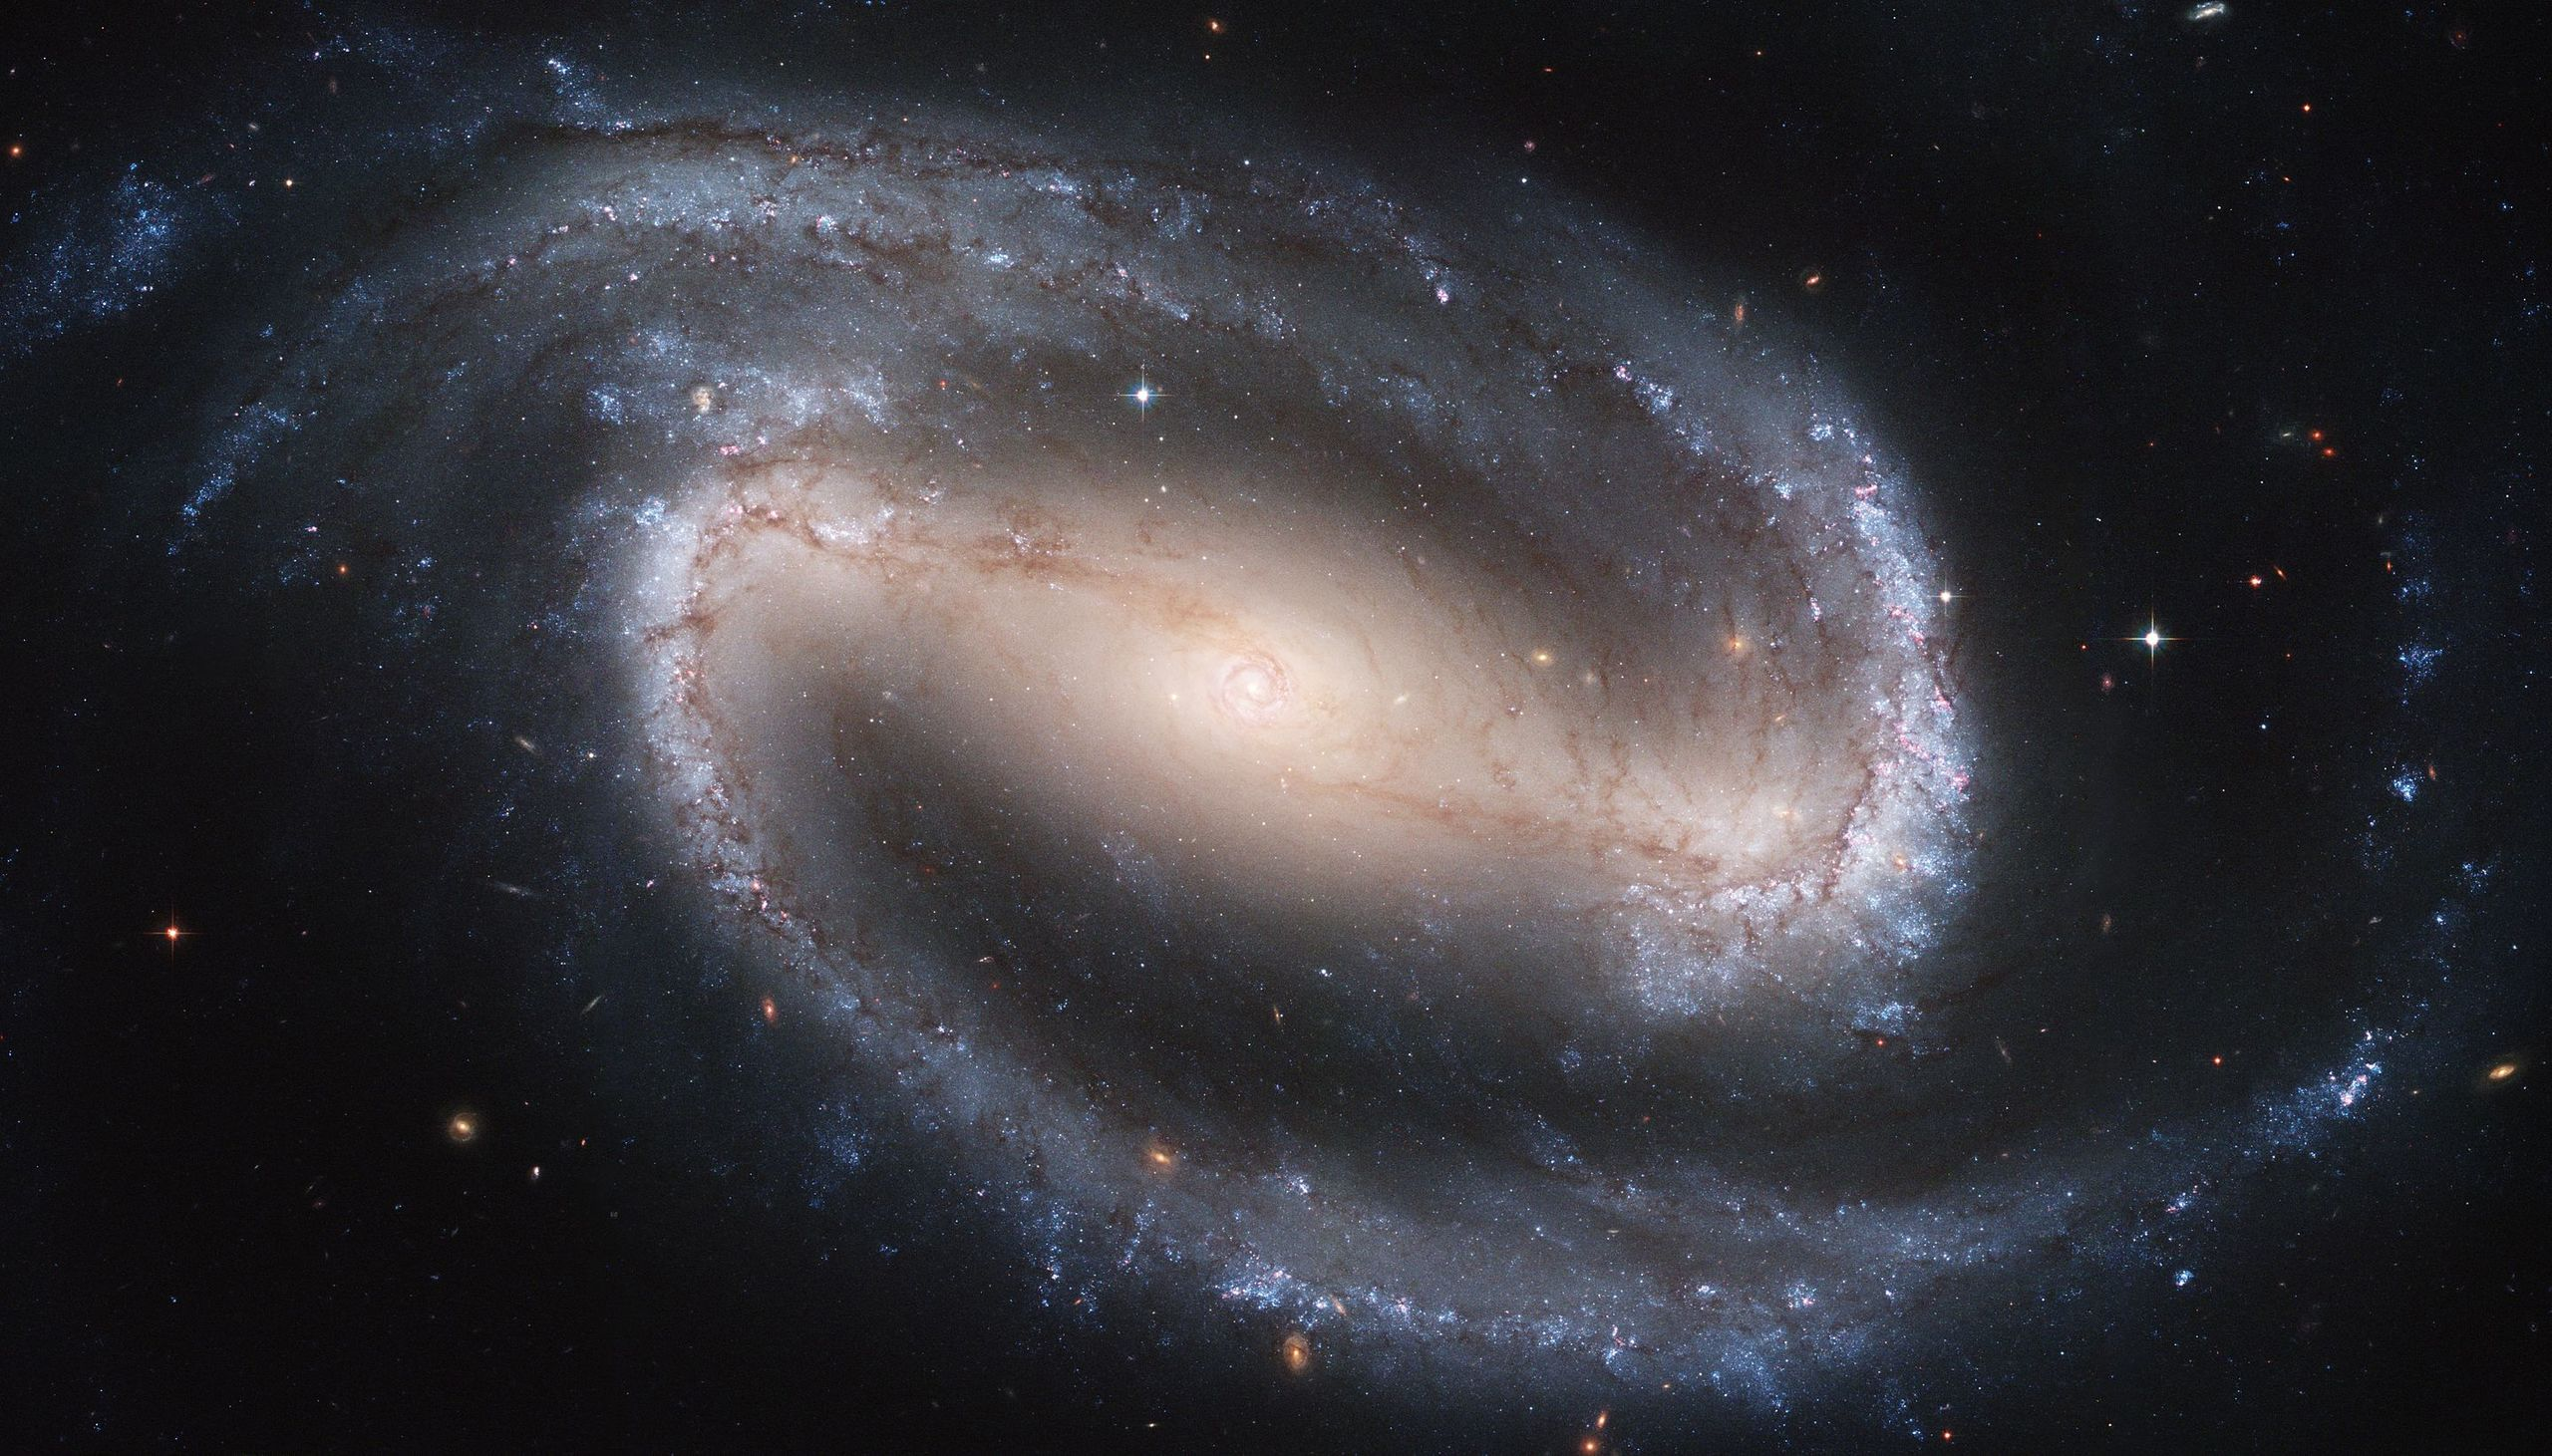
\includegraphics{figures/Hubble2005-01-barred-spiral-galaxy-NGC1300}}
\end{center}

\begin{flushright}
{ \tiny \em -- HST/STScI/NASA }
\end{flushright}

\vfill
\end{slide}

%------------------------------------------------------------------------------
\begin{slide}
\begin{center}
{\large \color{red} 
                  Barred Galaxies (NGC 1300, NGC 1073, ...)  }
\end{center}

\begin{itemize}
\item Example: NGC 1300. The most striking feature is the {\bf bar},
spanning almost the diameter of the galaxy. Two spiral arms are very
symmetrical. They can be followed almost for a full circle (on deep images).
This particular galaxy is a {\em grand-design spiral}.

\item Note that there are sharp, straight, dust lanes spanning the length of
the bar. The spiral arms start at the tips of the bar. At the start of each
spiral arm, there is a cluster of HII regions (i.e., rapid star formation is
occuring). {\bf These are all common features in barred spiral galaxies.}

\item Bars are a source of strong, asymmetric, perturbations. The disk responds
to these by creating spiral arms.

\end{itemize}

\vfill
\end{slide}


%------------------------------------------------------------------------------
\begin{slide}
\begin{center}
{\large \color{red} 
                  Barred Galaxies  }
\end{center}

Bars show up in a variety of sizes. They vary from dominating the appearance
of the disk, to weak oval distortions that are only visible in careful
Fourier decompositions of the light distribution.

They're typically quite elongated ($\sim 2:1$ ratios are seen in the
equatorial plane for SB galaxies).

The global fraction of disk galaxies varies on the exact criteria used;
classification by eye shows that 30\% to 50\% of spiral galaxies are
strongly barred in the optical\footnote{Where the size of the bar is
at least 30\% of the galaxy's diameter}.

The Milky Way, LMC and SMC are all barred.

\vfill
\end{slide}

%------------------------------------------------------------------------------
\begin{slide}
\begin{center}
{\large \color{red} 
                  Barred Galaxies  }
\end{center}

Bars are more prominent in Near-IR (Eskridge et al. 2000). As we've
discussed earlier, this implies they're a true density distortion. They show
typical bar-interbar ratios of $K \eqsim 3-6$.

Prominent dust lanes are found in bars, slightly offset in the direction of
rotation. There's observational evidence the gas and dust in these lanes is
highly compressed and shocked.

But apart from the presence of the bar (and the effects it causes), there
are few systemtic differences between barred and unbarred disk galaxies.

\vfill
\end{slide}


%------------------------------------------------------------------------------
\begin{slide}
\begin{center}
{\large \color{red} 
                  Dynamics of Bars  }
\end{center}

The bar pattern speed $\Omega_b$ is usually parametrized by the ratio
\eq{
	\mathcal{R} = \frac{R_{CR}}{a_0}
}
of the corotation radius to the bar semi-major axis. Dynamical arguments
show that weak bars must have $\mathcal{R} > 1$ (should not extend beyond
corotation).

Bars are often called ``fast'' if $\mathcal{R} \approx 1$ and ``slow'' if
$\mathcal{R} \gg 1$.  Observational evidence shows that, within the error
bars, all bars have $0.9 \lesssim \mathcal{R} \lesssim 1.3$ and {\bf are
therefore considered fast}. This is consistent with results from
numerical modeling.

This result has physical significance, as galaxies whose mass within the
disk radius is dominated by a dark halo are expected to have {\em slow}
bars. $\Rightarrow$ disk galaxies are baryion-dominated in their centers.

\vfill
\end{slide}





%------------------------------------------------------------------------------
%\begin{slide}
%
%\begin{center}
%{\large \color{red} 
%                 Effect of Perturbations on Stellar Disks }
%\end{center}
%
%If we perturb the axisymmetric potential of a rotating disk with
%a small non-axisymmetric component as above, it makes sense
%to define the angular speed of that perturbation as the frame
%speed. We call this the {\bf pattern speed}, $\Omega_p$.
%
%This potential is $m$-fold symmetric and may arise from a central
%bar pattern ($m=2$), an triaxial dark halo ($m=2$), some external
%perturbing agent such as a companion galaxy ($m=1$), or from
%large local mass concentrations within the disk of the galaxy
%($m=many$).
%
%At the corotation radius circularly orbiting particles feel a time-steady
%potential. In the case of an $m=2$ bar potential, a coresonant
%particle would perform small epicyclic orbits around a gyration
%point having constant phase and radial relationship with
%the bar.
%
%\end{slide}
%
%
%%------------------------------------------------------------------------------
%\begin{slide}
%
%\begin{center}
%{\large \color{red} 
%                 Resonances with the Rotating Pattern }
%\end{center}
%
%Particles at this radius feel an enhanced potential over their entire
%orbits. Since gravitational potentials are always attractive, this
%represents a barrier in the effective potential and is known as the
%{\bf corotation resonance} (CR).
%
%Two other resonances, discovered by and named after Lindblad,
%lie interior and exterior to the CR. These are the {\bf Inner and Outer
%Lindblad Resonances}, ILR and OLR.
%
%The dispersion relations that follow from instability analysis relate
%the wavenumber $k$ to the frequency $\omega$ ($\omega = m \Omega_p$).
%For CR, $\Omega = \Omega_p$, and for Lindblad resonances:
%\eq{
%	\Omega = \Omega_p \pm \frac{\kappa}{m}
%}
%
%\end{slide}
%
%%------------------------------------------------------------------------------
%\begin{slide}
%
%\begin{center}
%{\large \color{red} 
%                 The Region where Spiral Structure is Possible }
%\end{center}
%
%\begin{center}
%\scalebox{1}{\hskip 0.0in 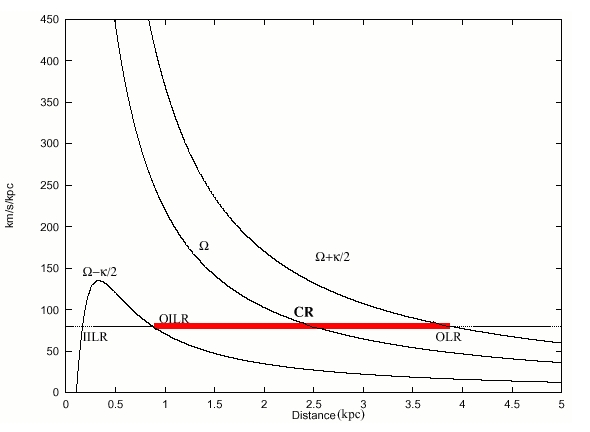
\includegraphics{figures/resonances}}
%\end{center}
%
%\end{slide}
%
%
%%------------------------------------------------------------------------------
%\begin{slide}
%
%A a particle at the Inner Lindblad Resonance (ILR) it is at
%the top of its epicycle when the end of the bar swings by
%below it, and will be at the top of its next epicycle when the
%opposite end of the bar swings by. The particle is oscillating
%radially at an integral multiple of the driving frequency and
%at a constant phase, which represents a condition of forced
%oscillation. This is another barrier in the effective potential.
%
%The Outer Lindblad Resonance (OLR) is similar except that
%particles are moving relatively retrograde from the rotating
%bar. Both resonances present barriers to the radial potential
%profile in the disk.
%
%{\bf $\Rightarrow$ Waves are trapped in the annular regions between Lindblad
%resonances.}
%
%Not all galaxies have inner Lindblad radii. The necessary
%condition for the formation of an ILR is a relatively rapid
%transition from a region of solid-body rotation to one of differential
%rotation (e.g. a flat rotation curve)
%
%\end{slide}

\end{document}


